%&pdflatex
\documentclass{elsarticle}

\usepackage{array}
\usepackage{amsmath,amssymb,amsfonts,amsthm}
\usepackage{mathtools}
\usepackage{algorithm, algorithmic}
\usepackage{graphicx}
\usepackage{subfigure}
\usepackage{color}
\usepackage{undertilde}
\usepackage[colorlinks = true, filecolor = red, urlcolor = blue, linkcolor = black]{hyperref}

\setlength\textwidth{6in}
\setlength\textheight{8in}
\setlength\oddsidemargin{0.25in} % LaTeX adds a default 1in to this!
\setlength\evensidemargin{0.25in}
\setlength\topmargin{-0.0in} % LaTeX adds a default 1in to this!
\setlength\headsep{0in}
\setlength\headheight{0in}
\setlength\footskip{1in}

\renewcommand{\topfraction}{0.85}
\renewcommand{\textfraction}{0.1}
\renewcommand{\floatpagefraction}{0.75}

\newcommand{\vect}[1]{\ensuremath\boldsymbol{#1}}
\newcommand{\tensor}[1]{\underline{\vect{#1}}}
\newcommand{\del}{\triangle}
\newcommand{\grad}{\nabla}
\newcommand{\curl}{\grad \times}
\renewcommand{\div}{\grad \cdot}
\newcommand{\ip}[1]{\left\langle #1 \right\rangle}
\newcommand{\eip}[1]{a\left( #1 \right)}
\newcommand{\pd}[2]{\frac{\partial#1}{\partial#2}}
\newcommand{\pdd}[2]{\frac{\partial^2#1}{\partial#2^2}}

\newcommand{\Reyn}{\rm Re}

\newcommand{\bs}[1]{\boldsymbol{#1}}
\DeclareMathOperator{\diag}{diag}

\newcommand{\equaldef}{\stackrel{\mathrm{def}}{=}}

\newcommand{\tablab}[1]{\label{tab:#1}}
\newcommand{\tabref}[1]{Table~\ref{tab:#1}}

\newtheorem{remark}{Remark}

\newcommand{\theolab}[1]{\label{theo:#1}}
\newcommand{\theoref}[1]{\ref{theo:#1}}
\newcommand{\eqnlab}[1]{\label{eq:#1}}
\newcommand{\eqnref}[1]{\eqref{eq:#1}}
\newcommand{\seclab}[1]{\label{sec:#1}}
\newcommand{\secref}[1]{\ref{sec:#1}}
\newcommand{\lemlab}[1]{\label{lem:#1}}
\newcommand{\lemref}[1]{\ref{lem:#1}}

\newcommand{\mb}[1]{\mathbf{#1}}
\newcommand{\mbb}[1]{\mathbb{#1}}
\newcommand{\mc}[1]{\mathcal{#1}}
\newcommand{\nor}[1]{\left\| #1 \right\|}
\newcommand{\snor}[1]{\left| #1 \right|}
\newcommand{\LRp}[1]{\left( #1 \right)}
\newcommand{\LRs}[1]{\left[ #1 \right]}
\newcommand{\LRa}[1]{\left\langle #1 \right\rangle}
\newcommand{\LRc}[1]{\left\{ #1 \right\}}
\newcommand{\LRb}[1]{\left| #1 \right|}

\newcommand{\Grad} {\ensuremath{\nabla}}
\newcommand{\Div} {\ensuremath{\nabla\cdot}}
\newcommand{\Nel} {\ensuremath{{N^\text{el}}}}
\newcommand{\jump}[1] {\ensuremath{\LRs{\![#1]\!}}}
\newcommand{\uh}{\widehat{u}}
\newcommand{\fnh}{\widehat{f}_n}
\renewcommand{\L}{L^2\LRp{\Omega}}
\newcommand{\pO}{\partial\Omega}
\newcommand{\Gh}{\Gamma_h}
\newcommand{\Gm}{\Gamma_{-}}
\newcommand{\Gp}{\Gamma_{+}}
\newcommand{\Go}{\Gamma_0}
\newcommand{\Oh}{\Omega_h}

\newcommand{\eval}[2][\right]{\relax
  \ifx#1\right\relax \left.\fi#2#1\rvert}

\def\etal{{\it et al.~}}


\def\arr#1#2#3#4{\left[
\begin{array}{cc}
#1 & #2\\
#3 & #4\\
\end{array}
\right]}
\def\vecttwo#1#2{\left[
\begin{array}{c}
#1\\
#2\\
\end{array}
\right]}
\def\vectthree#1#2#3{\left[
\begin{array}{c}
#1\\
#2\\
#3\\
\end{array}
\right]}
\def\vectfour#1#2#3#4{\left[
\begin{array}{c}
#1\\
#2\\
#3\\
#4\\
\end{array}
\right]}
\date{}

\newtheorem{proposition}{Proposition}
\newtheorem{corollary}{Corollary}
\newtheorem{theorem}{Theorem}
\newtheorem{lemma}{Lemma}

\newcommand{\G} {\Gamma}
\newcommand{\Gin} {\Gamma_{in}}
\newcommand{\Gout} {\Gamma_{out}}

%%%%%%%%%%%%%%% End def of new commands %%%%%%%%%%%%%%%%%%%
%%%%%%%%%%%%%%% Start of thesis %%%%%%%%%%%%%%%%%%%

\begin{document}
\begin{frontmatter}

\author{Jesse Chan\corref{cor1}}
\ead{jchan@ices.utexas.edu}
\cortext[cor1]{Principal Corresponding Author, Institute for Computational Engineering and Sciences, The University of Texas at Austin}
\cortext[affil]{Institute for Computational Engineering and Sciences, The University of Texas at Austin}
\author{Leszek Demkowicz\corref{affil}}
\ead{leszek@ices.utexas.edu}
\author{Robert Moser\corref{affil}}
\ead{rmoser@ices.utexas.edu}

\title{A DPG method for steady viscous compressible flow}

\begin{abstract}
The Discontinuous Petrov-Galerkin (DPG) method is a class of novel higher order adaptive finite element methods derived from the minimization of the residual of the variational problem \cite{DPG2}, and has been shown to deliver a method for convection-diffusion that is provably robust in the diffusion parameter \cite{DPGrobustness,DPGrobustness2}.  In this work, the DPG method is extrapolated to nonlinear systems, and applied to several problems in fluid dynamics whose solutions exhibit boundary layers or singularities in stresses.  In particular, the effectiveness of DPG as a numerical method for compressible flow is assessed with the application of DPG to two model problems over a range of Mach numbers and laminar Reynolds numbers using automatic adaptivity for higher order elements, beginning with highly under-resolved coarse initial meshes.  
\end{abstract}

\end{frontmatter}

%\maketitle

%\tableofcontents

\section{Introduction}

Standard numerical methods tend to perform poorly across the board for the class of PDEs known as singular perturbation problems; these problems are often characterized by a parameter that may be either very small or very large.  An additional complication of singular perturbation problems is that very often, in the limiting case of the parameter blowing up or decreasing to zero, the PDE itself will change types (e.g.\ from elliptic to hyperbolic).  A canonical example of a singularly perturbed problem is the convection-diffusion equation in domain $\Omega \subset \mathbb{R}^3$,
\[
\div \left(\beta u\right) - \epsilon \Delta u = f.
\]
The equation models the steady-state distribution of the scalar quantity $u$, representing the concentration of a quantity in a given medium, taking into account both convective and diffusive effects. Vector $\beta \in \mathbb{R}^3$ specifies the direction and magnitude of convection, while the singular perturbation parameter $\epsilon$ represents the diffusivity of the medium. In the limit of an inviscid medium as $\epsilon\rightarrow 0$, the equation changes types, from elliptic to hyperbolic, and from second order to first order.

%We will illustrate the issues associated with numerical methods for this equation using one dimensional examples.  In 1D, the convection-diffusion equation is
%\begin{align*}
%\beta u'-\epsilon u'' &= f.
%\end{align*}
%For Dirichlet boundary conditions $u(0)=u_0$ and $u(1)= u_1$, the solution 
%can develop sharp boundary layers of width $\epsilon$ near the outflow boundary.
%\begin{figure}[!h]
%\centering
%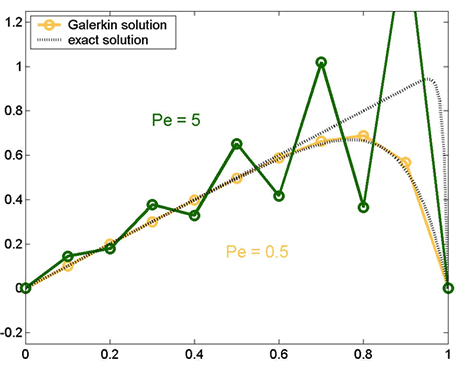
\includegraphics[width=2.5in]{figs/GalerkinOscTight.png}
%\caption{Oscillations in the 1D finite element solution of the convection-diffusion equation for small diffusion \cite{GalerkinOsc}. Standard finite volume and finite difference methods exhibit similar behavior.}
%\label{fig:GalerkinOsc}
%\end{figure}
The standard finite element method applied to the convection-dominated diffusion problem can perform very poorly for the case of small $\epsilon$.\footnote{This is especially true in the presence of boundary layers in the solution \cite{roos2008robust}.}  This poor performance can be observed numerically -- as the singular perturbation parameter $\epsilon$ decreases, the finite element solution can diverge significantly from the best finite element approximation of the solution.  
%The poor performance of the finite element method for this problem is reflected in the bound on the error in the finite element solution --- under the standard Bubnov-Galerkin method with $u\in H^1(0,1)$, we have the bound given in \cite{roos2008robust}:
%\[
%\|u-u_h\|_\epsilon \leq C \inf_{w_h}\|u-w_h\|_{H^1(0,1)},
%\]
%for $\|u\|_\epsilon^2 \coloneqq \|u\|_{L^2}^2 + \epsilon \|u'\|_{L^2}^2$, with $C$ independent of $\epsilon$. An alternative formulation of the above bound is 
%\[
%\|u-u_h\|_{H^1(0,1)} \leq C(\epsilon) \inf_{w_h}\|u-w_h\|_{H^1(0,1)},
%\]
%where $C(\epsilon)$ grows as $\epsilon\rightarrow 0$. The dependence of the constant $C$ on $\epsilon$ is what we refer to as a \textit{loss of robustness} --- as the singular perturbation parameter $\epsilon$ decreases, our finite element error is bounded more and more loosely by the best approximation error.  As a consequence, the finite element solution can diverge significantly from the best finite element approximation of the solution for very small values of $\epsilon$.  
For example, it is well known that, on a fixed coarse mesh and for small values of $\epsilon$ (or a large Peclet number, the ratio $h/\epsilon$), the Galerkin approximation of the solution to the convection-diffusion equation with a boundary layer develops spurious oscillations everywhere in the domain, even where the best approximation error is small.  These oscillations grow in magnitude as $\epsilon \rightarrow 0$, eventually polluting the entire solution.\footnote{For nonlinear shock problems, the solution often exhibits sharp gradients or discontinuities, around which the solution would develop spurious Gibbs-type oscillations. These are a result of underresolution of the solution, and are separate from the oscillations resulting from a lack of robustness.}  

Traditionally, instability/loss of robustness in finite element methods has been dealt with using residual-based stabilization techniques.  Given some variational form, the problem is modified by adding to the bilinear form the strong form of the residual, weighted by a test function and scaled by a stabilization constant $\tau$.  The most well-known example of this technique is the streamline-upwind Petrov-Galerkin (SUPG) method, which is a stabilized FE method for solving the convection-diffusion equation using piecewise linear continuous finite elements \cite{SUPG}.  SUPG stabilization not only removes the spurious oscillations from the finite element solution of the convection-diffusion equation, but delivers the best finite element approximation in the $H^1$ norm in 1D.  

From the perspective of the compressible Navier-Stokes equations, this loss of robustness is doubly problematic.  Not only will any nonlinear solution suffer from similar unstable oscillations, but nonlinear solvers themselves may fail to yield a solution due to such instabilities.  A nonlinear solution is almost always computed by solving a series of linear problems whose solutions will converge to the nonlinear solution under appropriate assumptions, and the presence of such oscillations in each linear problem can cause the solution convergence to slow significantly or even diverge.  Artificial viscosity and shock capturing methods have been used to suppress such oscillations and regularize the problem.  While these methods will usually yield smooth and qualitatively resolved solutions, these methods are often overly diffusive, yielding results which are poor approximations of the true solution \cite{Gresho1981223}, though modern artificial viscosity and shock capturing schemes have improved greatly in recent years \cite{Barter,Guermond20114248}.  We have taken an alternative approach in this work, avoiding artificial diffusion and shock capturing for the moment.  

Our aim is to develop a stable, higher order scheme for the steady compressible laminar Navier-Stokes equations in transonic/supersonic regimes that is automatically adaptive beginning with very coarse meshes.  This requires that both the method and the refinement scheme to perform adequately on coarse meshes with high Peclet numbers -- in other words, that the adaptive method is robust in the diffusion parameter.  We construct such a method in this paper as follows: we begin by deriving the DPG method for linear problems, then constructing a DPG method for the scalar convection-diffusion equation that is robust for very small viscosities.  Unlike common adaptive methods in computational fluid dynamics, which often refine based on physical features (such as high gradients in the solution), adaptivity under this method is driven by the minimization of a residual, which measures error accurately even for highly underresolved meshes.  The DPG method for scalar convection-diffusion is then extrapolated to systems of nonlinear equations, and applied to the compressible Navier-Stokes equations.  Numerical experiments are given, demonstrating the robustness of the method and the effectiveness of automatic adaptivity for two model problems in viscous compressible flow. 


The Discontinuous Petrov-Galerkin (DPG) method of Demkowicz and Gopalakrishnan was first formulated in \cite{DPG1} as a scheme for the pure convection problem. The method demonstrated promise --- in particular, the method was able to achieve optimal convergence rates for the Peterson problem where standard DG methods were suboptimal. A breakthrough came in \cite{DPG2}, where the concept of locally-computable optimal test functions led to the development of the DPG method in its current form. Soon after, the DPG method was successfully applied to solve the convection-diffusion problem in the small-diffusion limit with $\epsilon = 1e-7$ \cite{DPG2,DPG3}. 

Historically, the name DPG was given by Bottasso, Micheletti, Sacco and Causin to their method for elliptic problems in \cite{BottassoMichelettiSacco02}. The method was then extended to other problems, including convection-diffusion, in \cite{BottassoMichelettiSacco05,CausinSacco05,CausinSaccoBottasso05}. The key point in the method of Bottasso et al.\ was their method of hybridization of fluxes. Whereas HDG methods identify an additional flux unknown on the boundary, the numerical flux coupling neighboring elements together is still typically computed in part by using contributions from interior degrees of freedom on neighboring elements. In the DPG formulation, all numerical fluxes are declared to be independent unknowns, leaving the interior field degrees of freedom completely uncoupled from element to element. This formulation is often referred to as the \emph{ultra-weak} variational formulation. 

Since its inception, the DPG method has been applied to a wide range of problems with great success, including elasticity \cite{DPGElasLocking}, thin body shell problems \cite{DPGElas}, the cloaking problem in electromagnetics \cite{DPGcloak}, both Helmholtz and elastic wave propagation problems \cite{DPG4}, and recently, the linear Stokes equation \cite{stokesDPG}. DPG has also been shown to be a generalization of several successful finite element methods --- comparisons between DPG and standard DG methods can be found in \cite{DPG1}, and more recently, several existing DG methods have been shown to be derivable using the DPG framework \cite{Bui-ThanhDemkowiczGhattas11a,DGDPG}. 

Detailed analysis of the energy setting and well-posedness of DPG has been done for the Poisson and convection-diffusion equations in \cite{analysisDPG}. The well-posedness of DPG has also recently been extended to the large class of Friedrichs systems in \cite{Bui-ThanhDemkowiczGhattas11b}. Significant efforts have also been made in demonstrating the robustness of the DPG method for singular perturbation problems, both in wave propagation \cite{DPG4,DPGwave} and convection-diffusion problems \cite{DPGrobustness, DPGrobustness2}. 

\subsection{Optimal Petrov-Galerkin methods}

\seclab{optimalTest} Petrov-Galerkin methods, in which the test space differs from the trial space, have been explored for over 30 years, beginning with the approximate symmetrization method of Barrett and
Morton~\cite{BARRETT01101981}. The idea was continued with the SUPG method of Hughes, and the characteristic Petrov-Galerkin approach of Demkowicz and Oden~\cite{Demkowicz1986188}, which introduced the
idea of tailoring the test space to change the norm in which a finite element method would converge.

The idea of optimal test functions was introduced by Demkowicz and Gopalakrishnan in \cite{DPG2}.  Conceptually, these optimal test functions are the natural result of the minimization of a residual corresponding to the operator form of a variational equation. The connection between stabilization and least squares/minimum residual methods has been observed previously \cite{GLS}. However, the method in \cite{DPG2} distinguishes itself by measuring the residual of the natural \textit{operator form of the equation}, which is posed in the dual space, and measured with the dual norm, as we now discuss. 	

Throughout this work, we assume that the trial space $U$ and test space $V$ are real Hilbert spaces, and denote $U'$ and $V'$ as the respective topological dual spaces. Let $U_h \subset U$ and $V_h\subset V$ be finite dimensional subsets. We are interested in the following problem: given $l \in V'$, find $u_h \in U_h$  such that 
%\begin{equation}
%\eqnlab{variationEq}
%\left\{
%  \begin{array}{l}
%    \text{Given } l \in V', \text{ find } u_h \in U_h  \text{ such that} \\ 
%    b(u_h,v_h) = l(v_h), \quad \forall v_h\in V_h,
%  \end{array}
%  \right.
%\end{equation}
\begin{align}
b(u_h,v_h) &= l(v_h), \quad \forall v_h\in V_h, \eqnlab{variationEq}
\end{align}
where $b\LRp{\cdot,\cdot}: U \times V \to \mbb{R}$ is a continuous
bilinear form.  $U$ is chosen to be some trial space of approximating functions, but $V_h$ is as of yet unspecified. Throughout this work, we suppose the variational problem \eqnref{variationEq} to be well-posed. 

We can identify a unique operator $B:U\rightarrow V'$ such that
\[
\langle Bu,v\rangle_V \coloneqq b(u,v), \quad u\in U, v\in V
\]
with $\LRa{\cdot, \cdot}_V$ denoting the duality pairing between $V'$ and $V$, to obtain the operator form of the continuous variational problem
\begin{equation}
\eqnlab{dualEq}
Bu = l \quad \text{in } V'.
\end{equation}
In other words, we can represent the continuous form of our variational equation
\eqnref{variationEq} equivalently as the operator equation \eqnref{dualEq} with values in the
dual space $V'$.  This motivates us to consider the conditions under which the solution to \eqnref{variationEq} is the solution to the minimum residual problem in $V'$ 
\[
u_h = \underset{u_h\in U_h}{\arg\min}\, J(u_h),
\]
where $J(w)$ is defined for $w\in U$ as 
\[
J(w) = \frac{1}{2}\|Bw-l\|_{V'}^2 \coloneqq\frac{1}{2} \sup_{v\in V\setminus\{0\}} \frac{| b(w,v)-l(v)|^2}{\nor{v}_V^2}.
\]
For convenience in writing, we will abuse the notation $\sup_{v \in V}$ to denote $\sup_{v\in V\setminus\{0\}}$ for the remainder of this work.

Let us define $R_V: V \to V'$ as the Riesz map, which identifies
elements of $V$ with elements of $V'$ by 
\[
\langle R_V v,\delta
v\rangle_V \coloneqq(v, \delta v)_V, \quad \forall \delta v \in V.
\]
Here, $(\cdot, \cdot)_V$ denotes the
inner product in $V$. As $R_V$ and its inverse, $R_V^{-1}$, are both
isometries, e.g.\ $\|f\|_{V'} = \|R_V^{-1} f\|_V, \forall f \in V'$, we
have
\begin{equation}
\eqnlab{minimization}
\min_{u_h\in U_h} J(u_h) = \frac{1}{2}\left\|Bu_h-l\right\|_{V'}^2 =  \frac{1}{2}\left\|R_V^{-1}(Bu_h-l)\right\|_V^2.
\end{equation}
The first order optimality condition for \eqnref{minimization} requires
the G\^ateaux derivative to be zero in all directions $\delta u \in U_h$, i.e.,
\begin{align*}
\left(R_V^{-1}(Bu_h-l),R_V^{-1}B\delta u\right)_V = 0, \quad \forall \delta u \in U. 
\end{align*}
We define, for a given $\delta u \in U$, the corresponding {\em optimal test function} $v_{\delta u}$
\begin{equation}
\eqnlab{optv}
v_{\delta u} \coloneqq R_V^{-1}B\delta u \quad  \text{in } V.
\end{equation} 
The optimality condition then becomes
\[
 \langle Bu_h-l, v_{\delta u}\rangle_V = 0, \quad \forall \delta u \in U
\]
which is exactly the standard variational equation in
 \eqnref{variationEq} with $v_{\delta u}$ as the test functions. We can define the optimal test space $V_{\rm opt} \coloneqq \{v_{\delta u} \text{ s.t. } \delta u\in U\}$. Thus, the solution of the variational problem \eqnref{variationEq} with test space $V_h = V_{\rm opt}$ minimizes the residual in the dual norm $\nor{Bu_h-l}_{V'}$. This is the key idea behind the concept of optimal test functions. 

Since $U_h \subset U$ is spanned by a finite number of basis functions $\LRc{\varphi_i}_{i=1}^N$, \eqnref{optv} allows us to compute (for each basis function) a corresponding optimal test function $v_{\varphi_i}$. The collection $\LRc{v_{\varphi_i}}_{i = 1}^N$ of optimal test functions then forms a basis for the optimal test space.  In order to express optimal test functions defined in \eqnref{optv} in a more familiar form, we take  $\delta u = \varphi$, a generic basis function in $U_h$, and rewrite \eqnref{optv} as
\[
R_Vv_{\varphi} = B\varphi, \quad \text{in } V',
\]
which is, by definition, equivalent to
\[
\LRp{v_\varphi,\delta v}_V = \LRa{R_Vv_\varphi,\delta v}_{V}=
\LRa{B\varphi, \delta v}_V = b\LRp{\varphi,\delta v}, \quad
\forall \delta v \in V.
\]
%% Now, let us define the \textit{trial-to-test} operator $T =
%% R_V^{-1}B$, which, by \eqnref{optv}, maps a trial function $\delta u$
%% to its corresponding \textit{optimal} test function $v = T\delta u$.
%% On the other hand,
As a result, optimal test functions can be determined by solving the auxiliary
variational problem
\begin{equation}
\eqnlab{optvVar}
\left(v_\varphi,\delta v\right)_V = b(\varphi,\delta v), \quad \forall
\delta v \in V.
\end{equation}
However, in general, for standard $H^1$ and $H({\rm div})$-conforming finite element methods, test functions are continuous over the entire domain, and hence solving variational problem \eqnref{optvVar} for each optimal test function requires a global operation over the entire mesh, rendering the method impractical. A breakthrough came through the development of
discontinous Galerkin (DG) methods, for which basis functions are
discontinuous over elements. In particular, the use of discontinuous
test functions $\delta v$ reduces the problem of determining global 
optimal test functions
in \eqnref{optvVar} to local problems that can be solved in an
element-by-element fashion.

We note that solving \eqnref{optvVar} on each element exactly is
infeasible since it amounts to inverting the Riesz map $R_V$ exactly.
Instead, optimal test functions are approximated using the standard
Bubnov-Galerkin method on an ``enriched" subspace $\tilde{V} \subset
V$ such that $\dim(\tilde{V}) > \dim(U_h)$ elementwise \cite{DPG1, DPG2}. In this
document, we assume the error in approximating the optimal test functions
is negligible, and refer to the work in \cite{practicalDPG} for
estimating the effects of approximation error on the performance of DPG.

It is now well known that the DPG method
delivers the best approximation error in the ``energy norm" --- that is
\cite{Bui-ThanhDemkowiczGhattas11a, DPG2,DPG4} 
\begin{equation}
\eqnlab{optimalError}
\nor{u-u_h}_{U,E} = \inf_{w\in U_h} \nor{u-w}_{U,E},
\end{equation}
where the energy norm $\|\cdot \|_{U,E}$ is defined for a function $\varphi \in U$ as
\begin{equation}
\eqnlab{energyNorm} \|\varphi\|_{U,E} \coloneqq \sup_{v\in V}
\frac{b(\varphi,v)}{\|v\|_V} = \sup_{\nor{v}_V = 1} b(\varphi,v) =
\sup_{\nor{v}_V = 1} \LRa{B\varphi,v}_V = \nor{B\varphi}_{V'} =
\nor{v_\varphi}_V,
\end{equation}
where the last equality holds due to the isometry of the Riesz map
$R_V$ (or directly from \eqnref{optvVar} by taking the supremum). An
additional consequence of adopting such an energy norm is that,
without knowing the exact solution, the energy error $\|u-u_h\|_{U,E}$ can
be determined by computing $\|v_{u-u_h}\|_V$ from the following
identity
\[
\left(v_{u-u_h},\delta v\right)_V = b(u-u_h,\delta v) = l\LRp{\delta
v} - b(u_h,\delta v).
\]
This is simply a consequence of the minimum-residual nature of DPG; the energy error is simply the norm of the  residual in $V'$. 

Practically speaking, this implies that the DPG method is not only discretely stable, but delivers the \emph{best approximation in the energy norm} on any mesh. In particular, the stability and optimality of DPG apply naturally to higher order adaptive meshes, where discrete stability is often an issue. 

\subsection{Ultra-weak variational formulation}
\seclab{abstractUweak}

The naming of the discontinuous Petrov-Galerkin method refers to the fact that the method is a Petrov-Galerkin method, and that the test functions are specified to be discontinuous across element boundaries. There is no specification of the regularity of the trial space, and we stress that the idea of DPG is not inherently tied to a single variational formulation \cite{Bui-ThanhDemkowiczGhattas11a}. 

In most of the DPG literature, however, the discontinuous Petrov-Galerkin method refers to the combination of the concept of locally computable optimal test functions in Section \secref{optimalTest} with the so-called ``ultra-weak formulation" \cite{DPG1,DPG2,DPG3,DPG4,DPGElas,DBLP:journals/procedia/NiemiCC11}. Unlike the previous two sections in which we studied the general equation \eqnref{variationEq} given by abstract bilinear and linear forms, we now consider a concrete instance of \eqnref{variationEq} resulting from an ultra-weak formulation for an abstract first-order system of PDEs $Au = f$. Additionally, from this section onwards, we will refer to DPG as the pairing of the ultra-weak variational formulation with the concept of locally computable optimal test functions. 

We begin by partitioning the domain of interest $\Omega$ into $\Nel$ non-overlapping elements $K_j, j = 1,\hdots,\Nel$ such that $\Oh = \cup_{j=1}^\Nel K_j$ and $\overline{\Omega} = \overline{\Omega}_h$. Here, $h$ is defined as $h= \max_{j\in \LRc{1,\hdots,\Nel}}\text{diam}\LRp{K_j}$.  We denote the mesh ``skeleton" by $\Gh = \cup_{j=1}^\Nel \partial K_j$; the set of all faces/edges $e$, each of which comes with a normal vector ${n}_e$. The internal skeleton is then defined as $\Gamma^0_h = \Gh \setminus \partial \Omega$. If a face/edge $e \in \Gh$ is the intersection of $\partial K_i$ and $\partial K_j$, $i \ne j$, we define the following jumps:
\[
\jump{v} = \text{sgn} \LRp{{n}^-}v^- + \text{sgn} \LRp{{n}^+}v^+, \quad
\jump{\tau \cdot n} = {n}^-\cdot \tau^- + {n}^+\cdot\tau^+,
\]
where
\[
\text{sgn}\LRp{{n}^{\pm}} =
\left\{
\begin{array}{ll}
1 & \text{if } {n}^{\pm} = {n}_e \\
-1 & \text{if } {n}^\pm = -{n}_e
\end{array}
\right..
\]
For $e$ belonging to the domain boundary $\partial \Omega$, we define
\[
\jump{v} = v, \quad
\jump{\tau \cdot n} = {n}_e\cdot \tau.
\]
Note that we allow arbitrariness in assigning ``-'' and ``+'' quantities to the adjacent elements $K_i$ and $K_j$.

The ultra-weak formulation for $Au = f$ on $\Oh$, ignoring boundary
conditions for now, reads
\begin{equation}
\eqnlab{uweak}
b\left(\left(u, \widehat{u}\right),v\right) \coloneqq \langle \widehat{u}, \jump{v}
\rangle_{\Gh} - (u,A_h^*v)_{\Oh}= \LRp{f,v}_{\Oh},
\end{equation}
where we have denoted $\LRa{\cdot,\cdot}_{\Gh}$ as the duality
pairing on $\Gh$, $\LRp{\cdot,\cdot}_{\Oh}$ the $L^2$-inner
product over $\Oh$, and $A_h^*$ the formal adjoint resulting from
element-wise integration by parts.  Occasionally, for simplicity in
writing, we will ignore the subscripts in the duality pairing and
$L^2$-inner product if they are $\Gh$ and $\Oh$. Both the
inner product and formal adjoint are understood to be taken
element-wise. Using the ultra-weak formulation, the regularity
requirement on solution variable $u$ is relaxed, that is, $u$ is now
square integrable for the ultra-weak formulation \eqnref{uweak} to be
meaningful, instead of being (weakly) differentiable.  The trade-off
is that $u$ does not admit a trace on $\Gh$ even though it did
originally. Consequently, we need to introduce an additional new
``trace'' variable $\widehat{u}$ in \eqnref{uweak}, that is defined only on
$\Gh$.

The energy setting is now clear; namely,
\[
u\in L^2\LRp{\Oh} \equiv L^2(\Omega), \quad v\in V=D(A^*_h), \quad
\widehat{u}\in \gamma(D(A)),
\]
where $D(A_h^*)$ denotes the broken graph space corresponding to $A_h^*$,
and $\gamma(D(A))$ the trace space (assumed to exist) of the graph space of
operator $A$. The first discussion of the well-posedness of DPG with the ultra-weak formulation can be found in \cite{analysisDPG}, where the proof is presented for the Poisson and convection-diffusion equations. A more comprehensive discussion of the abstract setting for DPG with the ultra-weak formulation using the graph space, as well as a more general proof of well-posedness, can be consulted in \cite{Bui-ThanhDemkowiczGhattas11b}. 

\subsection{Choices of test and trial norms}
\seclab{energyPair}

A clear property of the energy norm defined by \eqnref{energyNorm} is that the trial norm $\nor{\cdot}_{U,E}$ is induced by a given test norm. However, the reverse relationship holds as well; for any trial norm, the test norm that induces such a norm is recoverable through duality. We have a result, proved in \cite{Bui-ThanhDemkowiczGhattas11a}: assuming, for simplicity, that the bilinear form $b(u,v)$ is definite, given any norm $\nor{\cdot}_{U}$ on the trial space $U$, for $\varphi \in U$, we can represent $\nor{\varphi}_{U}$ via
\[
\nor{\varphi}_{U} = \sup_{v \in V}\frac{b\LRp{w,v}}{\nor{v}_{V,U}}.
\]
where $\nor{v}_{V,U}$ is defined through
\[
\nor{v}_{V,U} = \sup_{w \in U}\frac{b\LRp{w,v}}{\nor{w}_{U}}.
\]
%In other words, the norm $\nor{\cdot}_V$ in $V$ can be recovered using the energy norm $\nor{\cdot}_{U,E}$ in $U$, and vice versa. 

In particular, given two arbitrary norms $\nor{\cdot}_{U,1}$ and $\nor{\cdot}_{U,2}$ in $U$
such that $\nor{\cdot}_{U,1} \le c \nor{\cdot}_{U,2}$ for some constant
$c$, they generate two norms $\nor{\cdot}_{V,U,1}$ and
$\nor{\cdot}_{V,U,2}$ in $V$ defined by
\[
\nor{v}_{V,U,1} \coloneqq \sup_{w \in U}\frac{b\LRp{w,v}}{\nor{w}_{U,1}}, \quad
\text{and }\nor{v}_{V,U,2} \coloneqq \sup_{w \in U}\frac{b\LRp{w,v}}{\nor{w}_{U,2}},
\]
such that $\nor{\cdot}_{V,U,1}$ and $\nor{\cdot}_{V,U,2}$ induce
$\nor{\cdot}_{U,1}$ and $\nor{\cdot}_{U,2}$ as energy
norms in $U$, respectively. That is,
\[
\|\varphi\|_{U,1} = \sup_{v\in V}
\frac{b(\varphi,v)}{\|v\|_{V,U,1}}, \quad \text{and }\|\varphi\|_{U,2} = \sup_{v\in V}
\frac{b(\varphi,v)}{\|v\|_{V,U,2}}.
\]

A question that remains to be addressed is to establish the relationship
between $\nor{\cdot}_{V,U,1}$ and $\nor{\cdot}_{V,U,2}$, given that
$\nor{\cdot}_{U,1} \le c \nor{\cdot}_{U,2}$. But this is
straightforward since we have
\begin{align*}
 \| v \|_{V,U,2} = \sup_{u \in U} \frac{b\left(w,v\right)}{\left\|
  w \right\|_{U,2}} \le c\sup_{w \in U} \frac{b\left(w,v\right)}{\left\| w
  \right\|_{U,1}} = c\| v \|_{V,U,1}.
\end{align*}
Consequently, a stronger energy norm in $U$ will generate a weaker
norm in $V$ and vice versa. In other words, to show that an
energy norm $\nor{\cdot}_{U,1}$ is weaker than another energy norm
$\nor{\cdot}_{U,2}$ in $U$, one simply needs to show the reverse inequality on the
corresponding norms in $V$, that is, $\nor{\cdot}_{V,U,1}$ is stronger
than $\nor{\cdot}_{V,U,2}$.

From now on, unless otherwise stated, we will refer to $\nor{\cdot}_{V,U}$ as the test norm that induces a given norm $\nor{\cdot}_U$. Likewise, we will refer $\nor{\cdot}_{U,V}$ as the trial norm induced by a given test norm $\nor{\cdot}_V$. In this work, for simplicity of exposition, we shall call a pair of norms in $U$ and $V$ that induce each other as an {\em energy norm pairing}.

From the discussion above of energy norm and test norm pairings, we know that specifying either a test norm or trial norm is sufficient to define an energy pairing. We now derive and discuss two important energy norm pairings, the first of which begins by specifying the canonical norm in $U$ and inducing a test norm on $V$. The second pairing begins instead by specifying the canonical norm on $V$ under the ultra-weak formulation \eqnref{uweak} and inducing an energy norm on the trial space $U$.

We begin first with the canonical norm in $U$. Since $\uh \in \gamma\LRp{D\LRp{A}}$, the standard norm for $\uh$ is
the so-called minimum energy extension norm defined as
\begin{equation}
\eqnlab{MEnorm}
\|\widehat{u}\| = \inf_{w\in D\LRp{A},
  \left.w\right|_{\Gh}=\widehat{u}} \|w\|_{D\LRp{A}}.
\end{equation}
The canonical norm for the group variable $\LRp{u,\uh}$ is then given by
\[
\|\left(u,\widehat{u}\right)\|_U^2 = \|u\|^2_{\L} + \|\widehat{u}\|^2,
\]
Applying the Cauchy-Schwarz inequality, we arrive at
\[
b\LRp{\LRp{u,\uh},v} \le \nor{\LRp{u,\uh}}_U \nor{v}_{V,U},
\]
where
\[
\nor{v}_{V,U}^2 = \|A_h^*v\|_{\L}^2
+\left(\sup_{\widehat{u} \in \gamma\LRp{D\LRp{A}}} \frac{\LRa{ \widehat{u},
  \jump{v} }_{\Gh}}{\|\widehat{u}\|}\right)^2.
\]

On the other hand, since $v \in D\LRp{A^*_h}$, the canonical norm for
$v$ is the broken graph norm: 
\[
\nor{v}_V^2 =  \|A_h^*v\|_{\L}^2 + \nor{v}_{\L}^2.
\]
Using the Cauchy-Schwarz inequality again, we obtain
\[
b\LRp{\LRp{u,\uh},v} \le \nor{\LRp{u,\uh}}_{U,V} \nor{v}_{V},
\]
where
\begin{equation}
\eqnlab{inducedQuasi}
\nor{\LRp{u,\uh}}_{U,V}^2 = \nor{u}_{\L}^2
+\sup_{v \in D\LRp{A_h^*}} \frac{\LRa{\widehat{u},
  \jump{v}}_{\Gh}^2}{\|v\|_V^2},
\end{equation}

Using the framework developed in \cite{Bui-ThanhDemkowiczGhattas11a},
one can show that both pairs $\LRp{\nor{\LRp{u,\uh}}_U,
  \nor{v}_{V,U}}$ and $\LRp{\nor{\LRp{u,\uh}}_{U,V}, \nor{v}_{V}}$ are
energy norm pairings in the sense discussed in Section
\secref{energyPair}. That is, the canonical norm $\nor{\LRp{u,\uh}}_U$
in $U$ induces (generates) the norm $\nor{v}_{V,U}$ in $V$, while the
canonical norm $\nor{v}_V$ in $V$ induces (generates) the energy norm
$\nor{\LRp{u,\uh}}_{U,V}$ in $U$. In the DPG literature \cite{DPG4}, $\nor{v}_{V,U}$ is known as the {\em optimal test norm},
while $\nor{v}_{V}$ is known as the {\em quasi-optimal test norm}.

\begin{figure}[!h]
\centering
\begin{tabular}{l c c}
Trial norm & & Test norm \\
\hline
$\boxed{\|u\|^2_{\L} + \|\widehat{u}\|^2}$ & $\Longrightarrow$  & $\|A_h^*v\|_{\L}^2
+\left(\sup_{\widehat{u}} \frac{\LRa{ \widehat{u},
  \jump{v} }_{\Gh}}{\|\widehat{u}\|}\right)^2$ \\
%\hline
%Quasi-optimal trial norm & & Canonical test norm \\
%\hline
$\nor{u}_{\L}^2+\sup_{v } \left(\frac{\LRa{\widehat{u},
  \jump{v}}_{\Gh}}{\|v\|_V}\right)^2$ &  $\Longleftarrow$ & $\boxed{\|A_h^*v\|_{\L}^2 + \nor{v}_{\L}^2}$
\end{tabular}
\caption{A summary of the derivation of test/trial norm pairings; we begin with the boxed norm on either the trial or test space, and induce the norm on the other space through duality. The optimal \textit{test} norm is naturally derived by beginning with the canonical norm on the trial space, while the quasi-optimal \textit{trial} norm is derived from beginning with the canonical norm on the test space.}
\end{figure}

The canonical norm $\nor{\LRp{u,\uh}}_U$ in $U$ provides a good
balance between the standard norms on the field $u$ and the flux
$\uh$ \cite{DPG4}. As a result, if the induced norm $\nor{v}_{V,U}$ (namely, the
optimal test norm) is used to compute  optimal test functions in
\eqnref{optvVar}, the finite element error in the canonical norm is the
best in the sense of \eqnref{optimalError}. 

Unfortunately, the optimal test norm is non-localizable due to the presence of the jump term $\jump{v}$.\footnote{A localizable norm can be written as $\nor{v}_{V(\Oh)} = \sum_{K\in\Oh} \nor{v}_{V(K)},$ where $\nor{v}_{V(K)}$ is a norm over $K$.} Since the jump terms couple elements together, the evaluation of the jump terms requires contributions from all the elements in the mesh. Consequently, solving for an optimal test function
amounts to inverting the Riesz map %, defined on the left sideof \eqnref{optvVar}, 
over the entire mesh $\Oh$, making the optimal test norm impractical.

On the other hand, the quasi-optimal test norm $\nor{v}_V$, namely the canonical norm in $V$, \textit{is} localizable, and hence practical. However, it's worth noting the difference between the induced energy norm $\nor{\LRp{u,\uh}}_{U,V}$ and the canonical norm in $U$; under the induced norm $\nor{\LRp{u,\uh}}_{U,V}$ there is no natural interpretation for the norm in which the error in the flux variable $\uh$ is measured. 

Using a variant of the quasi-optimal test norm, numerical results show that the DPG method appears to provide a ``pollution-free" method without phase error for the Helmholtz equation \cite{DPG4}, and analysis of the pollution-free nature of DPG is currently under investigation. Similar results have also been obtained in the context of elasticity \cite{DPGElas} and the linear Stokes equations \cite{Camellia}. On the theoretical side, the quasi-optimal test norm has been shown to yield a well-posed DPG methodology for the Poisson and convection-diffusion equations \cite{analysisDPG}. More recently, this theory has been generalized to show the well-posedness of DPG under the quasi-optimal test norm for the large class of Friedrichs' type PDEs \cite{Bui-ThanhDemkowiczGhattas11b}.  

\section{DPG for convection-diffusion}

The convection-diffusion problem can be given as a first order system: 
\begin{align*}
\div \left(\beta u - \sigma\right) &= f\\
\frac{1}{\epsilon}\sigma - \grad u &= 0,
\end{align*}
with inflow boundary conditions $\left.u\right|_{\Gamma_{\rm in}} = u_{\rm in}$, and outflow boundary conditions $\left.u\right|_{\Gamma_{\rm out}} = u_{\rm out}$.  The inflow and outflow boundaries are defined
\begin{align*}
\Gamma_{\rm in} &\coloneqq \{x\in \Gamma; \beta_n(x) \leq 0\}, \quad {\rm (inflow)}\\ 
\Gamma_{\rm out} &\coloneqq \{x\in \Gamma; \beta_n(x) > 0\}, \quad {\rm (outflow)}
%\Gamma_{0} &\coloneqq \{x\in \Gamma; \beta_n(x) = 0\},
\end{align*}
On domain $\Omega$, with mesh $\Oh$ and mesh skeleton $\Gh$, the ultra-weak variational formulation for convection-diffusion is
\begin{align*}
b\left(\left(u,\sigma, \widehat{u}, \widehat{f}_n\right),\left( v, \tau \right)\right) &= 
\left(u,\div \tau - \beta \cdot \grad v\right)_{\Oh} + \left(\sigma, \epsilon^{-1} \tau + \grad v\right)_{\Oh} 
- \LRa{\jump{\tau\cdot n}, \widehat{u} }_{\Gh} + \LRa{ \widehat{f}_n, \jump{v} }_{\Gh}.
\end{align*}
with $v\in H^1$ and $\tau \in H({\rm div},\Oh)$. 

\subsection{Inflow boundary condition and choice of test norm}
\seclab{sec:testNormSec}

Given the above properties of DPG, we can see that the choice of test norm will determine the behavior of DPG; however, the proper choice of test norm can be unclear.  There exists a canonical graph norm for the ultra-weak variational formulation under which well-posedness can be proven for a large class of problems, and near-optimality is observed in numerical experiments \cite{DPG4, Bui-ThanhDemkowiczGhattas11b, stokesDPG}.  However, for the specific problem of convection-diffusion, the resolution of optimal test functions resulting from the graph norm prove very difficult to approximate \cite{globalLocalDPG}.  In \cite{DPGrobustness}, Demkowicz and Heuer introduced guidelines for the construction of alternative test norms based on energy estimates for the adjoint equation. We follow \cite{DPGrobustness2}, where, in addition to constructing an alternative test norm, a new inflow boundary condition is introduced in order to regularize the adjoint equation.  

Typical boundary conditions for the convection-diffusion problem enforce a Dirichlet condition on both inflow and outflow.  We adopt instead a``conserved flux'' inflow boundary condition, 
\[
\beta_nu - \epsilon\pd{u}{n} \approx u_{\rm in}.
\]
This corresponds to the imposition of a boundary condition on the conserved flux $\fnh = \beta_nu - \sigma_n$.  For small $\epsilon$ and most problems of interest, both $\pd{u}{n}$ and $\epsilon$ tend to be small, such that the above is a good approximation of $\left.u\right|_{\Gamma_{\rm in}} = u_{\rm in}$.

Under this boundary condition, the adjoint problem is regularized such that its solutions are smoother, which in turn improves the stability of the DPG method \cite{DPGrobustness2}.  We illustrate this improvement with a simple numerical experiment; Figure~\ref{fig:confusion1D} demonstrates the behavior of the DPG method under both the standard Dirichlet and the new conserved flux boundary conditions.  In both cases, the test norm used is the 1D Sobolev norm $\nor{\LRp{v,\tau}}_V\coloneqq \nor{v}_{H^1} + \nor{\tau}_{H^1}$.  The left figure shows the behavior of DPG under a Dirichlet boundary condition; degeneration of the solution is observed as $\epsilon$ decreases.  In contrast, under the new conserved flux boundary condition, as $\epsilon$ decreases, the solution converges to the $L^2$ projection of the exact solution onto our trial space.  

\begin{figure}
\centering
\subfigure[Dirichlet boundary condition $u(0) = 1$]{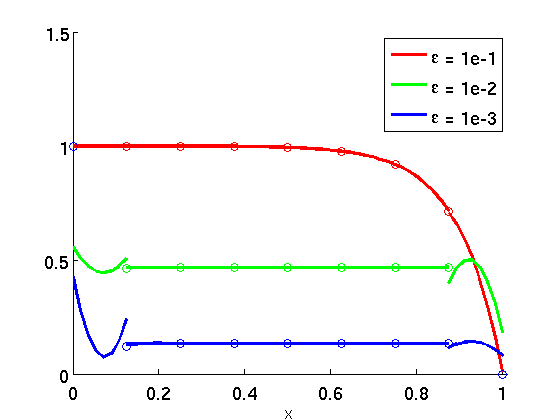
\includegraphics[width=2.75in]{dirichletBC.png}}
\subfigure[``Conserved flux'' boundary condition $u(0) - \epsilon u'(0) = 1$]{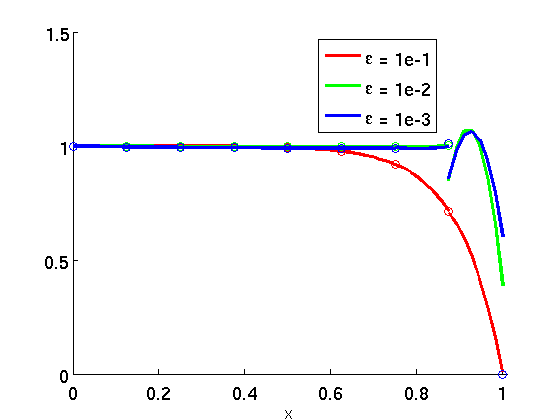
\includegraphics[width=2.75in]{newBC.png}}
\caption{Behavior of the 1D DPG method for convection diffusion under both standard Dirichlet and conserved flux boundary conditions.}
\label{fig:confusion1D}
\end{figure}

The test norm for convection-diffusion in multiple dimensions is defined elementwise on $K$ as
\[
\|\left(v,\tau\right)\|_{V,K}^2 = \min\left\{\frac{\epsilon}{|K|},1\right\}\|v\|^2 + \epsilon \|\grad v\|^2 + \|\beta \cdot \grad v\|^2 + \| \div \tau-\beta\cdot\grad v\|^2 + \min\left\{\frac{1}{\epsilon},\frac{1}{|K|}\right\}\|\tau\|^2.
\]
DPG under $\nor{\cdot}_V$ both delivers robust control of the $L^2$ error in the variables $u$ and $\sigma$ and minimizes approximation error in the solution of \eqnref{optvVar}.

\subsection{Anisotropic refinement}
\seclab{sec:aniso}
Isotropic adaptive mesh refinement has shown itself to be an effective way to resolve isolated solution features with large gradients, such as point singularities \cite{hp1,hp3}. However, for the resolution of phenomena such as shocks or boundary layers, anisotropic mesh refinement can resolve solution features for a much lower cost per degree-of-freedom, due to the fact that boundary layers in $n$-dimensions are primarily phenomena supported over $n-1$ dimensions.  

As a least squares method, DPG already includes a natural error indicator with which to drive adaptive mesh refinement.  To introduce anisotropic refinements, we need to introduce an anisotropy indicator in order to detect in which direction solution features are aligned.  In general, a test norm can be expressed as the sum of normed quantities, both scalar and vector valued.  If we restrict ourselves to quadrilateral elements for the moment, a general anisotropy indicator for DPG can be constructed by evaluating the $\L$ norms of the individual components of vector valued terms in the test norm.  

Under the robust test norm derived in this chapter for the convection-dominated diffusion problem, we can define $x$ and $y$ error contributions over a single element
\begin{align*}
e_{x,K} &= \epsilon \nor{\pd{v}{x}}_{L^2(K)}^2 + \nor{\tau_x}_{L^2(K)}^2 \\
e_{y,K} &= \epsilon \nor{\pd{v}{y}}_{L^2(K)}^2 + \nor{\tau_y}_{L^2(K)}^2.
\end{align*}
We define the anisotropy indicator as the ratio $r_K = \frac{e_{x,K}}{e_{y,K}}$, and implement a simple refinement scheme following \cite{DPG3}.  Given some anisotropic threshold $\epsilon_r$, if $r_K>\epsilon_r$, then we can conclude that the error in the $x$ direction is large compared to the $y$ direction, and we anisotropically refine the element along the $x$-axis.  Likewise, if $r_K < \frac{1}{\epsilon_r}$, this implies that the opposite is true, and we refine the element anisotropically along the $y$-axis.  

%We note that it is possible to compute the discrete system without needing much additional integration.  Recall that if we let $G$ be the symmetric positive-definite Gram matrix representing the inner product $\LRp{v,\delta v}_V$ on $V_h$, we solve for degrees of freedom $c_e$ representing our error representation function $e$.  
%
%For both the graph and robust test norms, we can decompose the inner product that induces the test norm into 
%\[
%\LRp{v,\delta v}_V = \sum_i \LRp{v,\delta v}_{V,x_i} + \LRp{v,\delta v}_{V,{\rm scalar}}
%\]
%such that $\LRp{v,\delta v}_{V,x_i}$ is a seminorm containing the $i$th coordinate component of a vector-valued test term, and $\LRp{v,\delta v}_{V,{\rm scalar}}$ is simply the non-vector portions of the test norm.  For example, if we take the $H^1(\Omega)$ Sobolev norm
%\[
%\LRp{v,\delta v}_V = \LRp{v,\delta v}_{\L} + \LRp{\grad v,\grad \delta v}_{\L}
%\]
%then $\LRp{v,\delta v}_{V,x_i} = \LRp{\pd{v}{x_i},\pd{\delta v}{x_i}}_{\L}$, and $\LRp{v,\delta v}_{V,{\rm scalar}} = \LRp{v,\delta v}_{\L}$.  Each bilinear term $\LRp{v,\delta v}_{V,x_i}$ induces a symmetric positive-semidefinite matrix $G_{x_i}$, such that 
%\[
%c_e^TG_{x_i}c_e = \nor{e}^2_{V,x_i}.
%\]
%By storing $G$ as the sum of $G_{\rm scalar}$ and $G_{x_i}$, we can then cheaply compute the anisotropic error indicators once we have the degrees of freedom corresponding to our error representation function.  



\section{DPG for nonlinear problems}

In this chapter, we extend DPG to the nonlinear setting and apply it to two problems in computational fluid dynamics.  We take as our starting point a nonlinear variational formulation
$b(u,v) = l(v)$, which is linear in $v$, but not in $u$.  An appropriate linearization gives
\[
b_u(\Delta u,v) = l(v) - b(u,v),
\]
where $b_u(\Delta u,v)$ is the linearization of $b(u,v)$ with respect to $u$.  Let $B(u)$ and $B_u\Delta u$ be the variational operators associated with $b(u,v)$ and $b_u(\Delta u,v)$, respectively.  We define two additional measures: 
\begin{align*}
\|\Delta u\|_E \coloneqq & \nor{B_u\Delta u}_{V'} = \nor{R_V^{-1} B_u\Delta u}_V = \sup_{v\in V} \frac{b_u(\Delta u,v)}{\nor{v}_V}\\
\nor{R(u)}_E \coloneqq & \nor{B(u)-l}_E = \nor{B(u) - l}_{V'}  = \nor{R_V^{-1} B(u)-l}_V = \sup_{v\in V} \frac{b(u,v)-l(v)}{\nor{v}_V}
\end{align*}
These two quantities are measures of the linearized update $\Delta u$ and the nonlinear residual in the appropriate norm in the dual space $V'$.  The first will be used to measure convergence of a nonlinear solution scheme to a stable discrete solution, while the second will be used to assess the convergence of the discrete solution to the continuous solution.  

\subsection{Nonlinear solution strategies}

The solution of a nonlinear problem is most commonly found using an iterative method, where a series of solutions to linear problems is expected to converge to the nonlinear solution.  We use two main methods to iterate to a nonlinear solution.  
\begin{itemize}
\item{} \textbf{(Damped) Newton iteration :} Given the linearized system $b_u(\Delta u,v) = b(u,v)-l(v)$, we begin with some initial guess $u\coloneqq u_0$ and solve for $\Delta u_0$.  The process is then repeated with $u\coloneqq u_{i+1} \coloneqq u_i + \alpha_i \Delta u_i$, where $\alpha_i \in (0,1]$ is some damping parameter that may limit the size of the Newton step in order to optimize the rate of convergence or preserve physicality of the solution.  The solution is considered converged when $\nor{\Delta u}_E \leq tol$.  
\item{} \textbf{Pseudo-time stepping: } An alternative method for the solution of steady-state systems is to use a pseudo-timestepping method.  The most common approach is to discretize the equations in time using a stable, implicit method --- if $Lu = f$ is our nonlinear problem and $L_u$ is the linearization of the nonlinear operator $L$ with respect to $u$, then the pseudo-timestepping method solves at each discrete time $t_{i}$
\[
\pd{u}{t} + Lu = f \rightarrow \frac{u(t_i) - u(t_{i-1})}{\Delta t} + L_{u(t_i)}\Delta u(t_i) = (f - Lu(t_i)).
\]
The solution at the next timestep is then set $u(t_{i+1}) \coloneqq u(t_i) + \Delta u(t_i)$.  This procedure is then repeated for the next timestep $t_{i+1}$ until the transient residual decreases such that $\nor{u(t_i) - u(t_{i-1})}_{L^2(\Omega)} = \nor{\Delta u(t_i)}_{L^2(\Omega)} \leq tol$.\footnote{Strictly speaking, seeking the solution at each timestep involves the solution of a nonlinear problem, requiring a Newton-type iteration to solve for $u(t_i)$.  However, for most applications, it is sufficient to approximate the nonlinear solution using a single Newton solve at each time step.} 
\end{itemize}

In practice, most compressible flow solvers opt for the pseudo-time step method over the direct Newton iteration due to the difficulty of convergence and sensitivity of the Newton iteration to initial guess\cite{libMeshPaper}.  Though the convergence of the pseudo-time step is slower, the addition of the zero-order transient terms ``regularizes" the problem and makes it less difficult to solve.\footnote{The addition of a zero-order term ``regularizes" an equation by adding to it a positive-definite $L^2$ projection operator.  In the limit as $\Delta t\rightarrow 0$, the solution at $t_i$ will simply return the $L^2$ projection of the solution at the previous timestep.}

A second class of nonlinear solvers are optimization methods.  Since DPG allows for the formulation of a discrete nonlinear residual, it is possible to formulate the nonlinear DPG problem as a minimization problem and use an optimization method to solve the discrete nonlinear problem.  This approach has been successfully implemented by Peraire et al.\ in solving compressible gas dynamics problems on uniform grids using a modified version of the ultra-weak variational formulation \cite{MITDPG}.  An additional advantage of such an approach would be the more direct enforcement of physical constraints, which are treated in an ad-hoc manner in most compressible Navier-Stokes solvers.  

\subsection{DPG as a nonlinear minimum residual method}

A recent theoretical development is the formulation of a DPG method that aims to minimize a nonlinear residual. Given two Hilbert spaces --- a trial space $U$ and test space $V$ --- our nonlinear variational formulation can be written as $b(u,v) = l(v)$, with the corresponding operator form of the formulation in $V'$
\[
B(u) = l.
\]
We can apply the steps used to derive the DPG method for linear problems to the nonlinear setting as well. Given a finite dimensional subspace $U_h \subset U$, we consider the discrete nonlinear residual
\[
J(u_h) \coloneqq \frac{1}{2}\nor{R_V^{-1}\left(B(u_h)-l\right)}_V^2.
\]
Our goal is to solve
\[
u_h = \arg \min_{w_h\in U_h}J(w_h).
\]
Similarly to the linear case, we can take the Gate\'aux derivative to arrive at a necessary condition for $u_h$ to minimize $J(u_h)$ 
\begin{align*}
\LRa{J'(u_h), \delta u_h} &= \LRp{R_V^{-1}\left(B(u_h)-l\right),R_V^{-1}B'(u_h;\delta u_h)}_V, \quad \delta u_h \in U_h. 
\end{align*}
As the above is a nonlinear equation, we seek its solution through linearization. Differentiating a second time in $u$, we arrive at
\begin{align*}
\LRa{J''(u_h), \Delta u_h} =& \LRa{B'(u_h;\Delta u_h), B'(u_h;\delta u_h)}_V \\
& + \LRa{\left(B(u_h)-l\right),B''(u_h;\delta u_h,\Delta u_h)}_V \\
=& \LRp{R_V^{-1}B'(u_h;\Delta u_h), R_V^{-1}B'(u_h;\delta u_h)}_V \\
& + \LRp{R_V^{-1}\left(B(u_h)-l\right),R_V^{-1}B''(u_h;\delta u_h,\Delta u_h)}_V 
\end{align*}
where $B''(u_h;\delta u_h,\Delta u_h)$ denotes the Hessian of $B(u_h)$, evaluated using both $\delta u_h$ and $\Delta u_h$. 

Examining the above formulation, we note that DPG as applied to the linearized problem produces the term $ \LRp{R_V^{-1}B'(u_h;\Delta u_h), R_V^{-1}B'(u_h;\delta u_h)}_V$. However, in approaching the nonlinear problem through the minimization of the discrete residual, we gain a second-order term involving the Hessian
\[
\LRp{R_V^{-1}\left(B(u_h)-l\right),R_V^{-1}B''(u_h;\delta u_h,\Delta u_h)}_V.
\] 
The evaluation of this term can be done in a computationally efficient manner --- if we define the image of the nonlinear residual under the Riesz inverse
\[
v_{R(u)} = R_V^{-1}\left(B(u_h)-l\right),
\]
then we can compute this additional term through
\begin{align*}
\LRp{v_{R(u)},R_V^{-1}B''(u_h;\delta u_h,\Delta u_h)}_V &= \LRa{v_{R(u)},B''(u_h;\delta u_h,\Delta u_h)}_V
\end{align*}
which can be computed in the same fashion as a Bubnov-Galerkin stiffness matrix. This addition, though not positive definite, is symmetric due to the nature of second order derivatives. 

We note that we have not implemented this Hessian-based nonlinear solver in the numerical experiments to follow, and instead plan to do so in the proposed work outlined in Section~\secref{sec:proposedWork}.


\section{The viscous Burgers equation}

We will illustrate the application of DPG to nonlinear problems using a viscous Burgers' equation on domain $\Omega = [0,1]^2 \in \mathbb{R}^2$
\[
\pd{\left(u^2/2\right)}{x} + \pd{u}{y} - \epsilon \Delta u = f.
\]
If we remove the viscous term, the above problem reduces to the form of the 1D transient Burgers equation, whose solution we can determine via the method of characteristics.  For boundary conditions 
\[
u(x.y) = 1-2x, \quad x = 0, y = 0,
\]
the solution forms a shock discontinuity starting at $(x,y) = (.5,.5)$, which then propagates upward in the $y$-direction.  The addition of the viscous term smears this discontinuity, leading to a solution with a smooth shock of width $\epsilon$.  

We begin by writing the equation in a first order system.  Defining $\beta(u) = \LRp{u/2,1}$, the above Burgers equation can be written as
\begin{align*}
\div\left(\beta(u)u-\sigma\right) &=f \\
\frac{1}{\epsilon}\sigma - \grad u &=0.
\end{align*}
Analogously to the convection-diffusion problem, the DPG nonlinear variational formulation can then be given
\[
b\left(\left(u,\sigma,\widehat{u},\widehat{f}_n\right),\left(v,\tau\right)\right) = \LRp{u,\div \tau - \beta(u) \cdot \grad v} + \LRp{\sigma, \frac{1}{\epsilon}\tau + \grad v} + \LRa{\widehat{u},\tau\cdot n} + \LRa{\widehat{f}_n,v} = \LRp{f,v}
\]
Linearizing the above then gives us 
\begin{align*}
b_u\left(\left(\Delta u,\sigma,\widehat{u},\widehat{f}_n\right),\left(v,\tau\right)\right) &= \LRp{\Delta u,\div \tau - \vecttwo{u}{1} \cdot \grad v} + \LRp{\sigma, \frac{1}{\epsilon}\tau + \grad v} + \LRa{\widehat{u},\tau\cdot n} + \LRa{\widehat{f}_n,v} \\
&= \LRp{u,\div \tau - \beta(u)\cdot \grad v} 
\end{align*}
Notice that the nonlinear term is only dependent on $u$, and thus there is no need to linearize in the variables $\sigma$, $\widehat{u}$, and $\widehat{f}_n$.  

Since the linearized Burgers' equation is of the form of a convection-diffusion problem with non-homogeneous load, we adopt the test norm described in Section~\secref{sec:testNormSec} with convection vector $\beta = (u,1)$.  

Recall that we did not linearize in the flux variables $\widehat{u}$ and $\widehat{f}_n$, so we can directly apply the nonlinear boundary conditions to our variational formulation.  Additionally, since Burgers' equation does not have any physical constraints, we can employ a direct Newton iteration to solve the nonlinear equation.  The adaptivity algorithm is identical to the greedy algorithm described previously, except that the linear solve is replaced by a nonlinear solve.  The results of an adaptive simulation are shown in Figure~\ref{fig:BurgersShock} for $\epsilon = 1e-4$.  

\begin{figure}[!h]
\centering
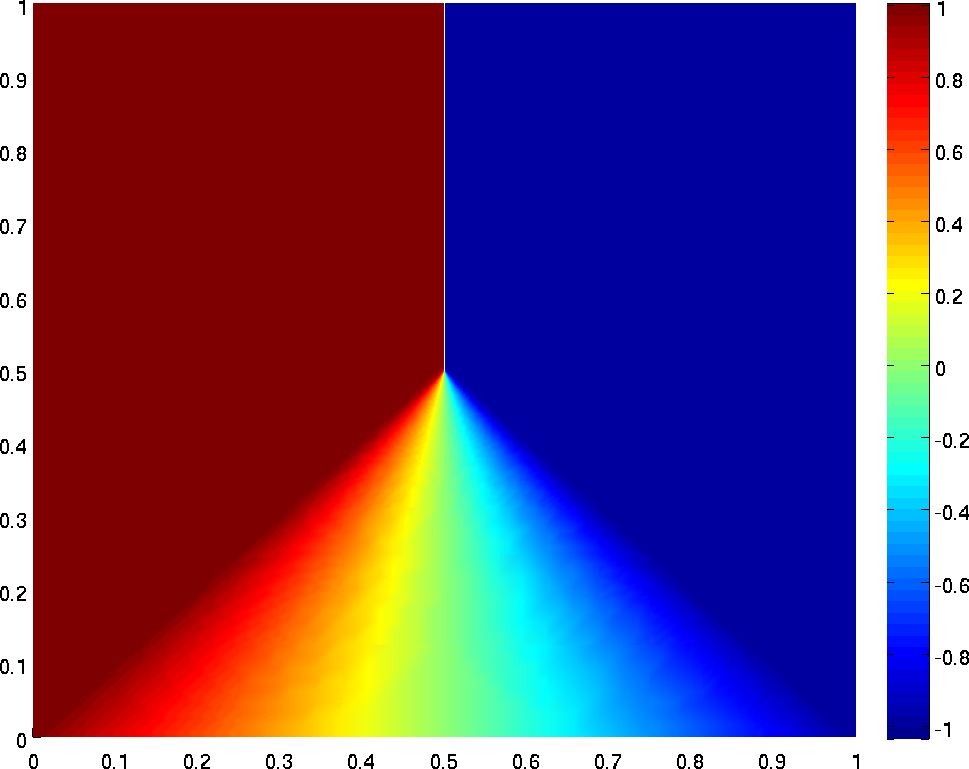
\includegraphics[scale=.5]{figs/burgers1e4.png}
\caption{Shock solution for Burgers' equation with $\epsilon = 10^{-4}$.} 
\label{fig:BurgersShock}
\end{figure}
\todo{Get mesh and zoomed in plot for Burgers' equation.} 


\section{The compressible Navier-Stokes equations}

We briefly review the compressible Navier-Stokes equations, given in Section~\secref{sec:compNS}, and formulate DPG for the nonlinear system. 
\begin{itemize}
\item \textbf{Conservation equations}
\begin{align*}
\div \vecttwo{\rho u_1 }{\rho u_2} &= 0\\
\div \vecttwo{\rho u_1^2+p }{\rho u_1 u_2} &= \div\left(\vec{\sigma_{i1}}\right)\\
\div \vecttwo{\rho u_1 u_2}{\rho u_2^2+p } &= \div\left(\vec{\sigma_{i2}}\right)\\
\div\vecttwo{((\rho e)+p)u_1}{((\rho e)+p)u_2} &= \div\left[\boldsymbol\sigma U + \vec{q}\right],
\end{align*}
where $\boldsymbol \sigma$ is the stress tensor whose $ij$th term is $\sigma_{ij}$.  

\item \textbf{Newtonian fluid laws}

We represent $\boldsymbol\sigma$ using the Newtonian fluid law
\[
\sigma_{ij} = \mu(u_{i,j} + u_{j,i}) + \lambda u_{k,k} \delta_{ij}
\]
where $\mu$ is viscosity and $\lambda$ is bulk viscosity. 
%Following elasticity, a general formula for the stress tensor is 
%\[
%\sigma_{ij} = 2\mu \epsilon_{ij} + \lambda \epsilon_{kk} \delta_{ij}
%\]
We can invert the stress tensor under isotropic and plane strain assumptions to get
\[
\frac{1}{2}\left(\grad  U + \grad ^T  U\right) = \frac{1}{2\mu} \sigma_{ij} - \frac{\lambda}{4\mu (\mu + \lambda)} \sigma_{kk}\delta_{ij}
\]
We also have
\[
\frac{1}{2}\left(\grad  U + \grad ^T  U\right) = \grad  U - \boldsymbol \omega
\]
where $\boldsymbol \omega$ is the antisymmetric part of the infinitesimal strain tensor:
\[
\boldsymbol \omega = \frac{1}{2}\left(\grad  U - \grad ^T  U\right).
\]
Thus our final form is
\begin{align*}
\grad  U - \boldsymbol \omega = \frac{1}{2\mu} \boldsymbol \sigma - \frac{\lambda}{4\mu (\mu + \lambda)} { \rm tr}(\boldsymbol \sigma) \boldsymbol I.
\end{align*}
Notice that $\boldsymbol \omega$ is implicitly defined to be the symmetric part of $\grad u$ by taking the symmetric part of the above equation. 

We note that, though this is a standard approach in solid mechanics, it is nonstandard compared to the usual finite element and DG approaches to the viscous stresses. We adopt such an approach to better mirror our experiences with the convection-diffusion equation \cite{DPGrobustness,DPGrobustness2}. 


\item \textbf{Fourier's heat conduction law}

We assume Fourier's law 
\begin{align*}
\vec{q} &= \kappa \grad T,
\end{align*}
%where $\kappa$ is generally a function of temperature. 
We introduce here the Prandtl number here as well
\[
{\rm Pr} = \frac{\gamma c_v \mu}{\kappa}.
\]
In this case, we assume a constant Prandlt number, which implies that the heat conductivity $\kappa$ is proportional to viscosity $\mu$.

\end{itemize}

\subsection{Nondimensionalization}
To nondimensionalize our equations, we introduce nondimensional quantities for length, density, velocity, temperature, and viscosity. 
\[
\boldsymbol x^* = \frac{\boldsymbol x}{L}, \qquad \rho^* = \frac{\rho}{\rho_{\infty}}, \qquad u_1^* = \frac{u_1}{V_\infty}, \qquad u_2^* = \frac{u_2}{V_\infty}, \qquad T^* = \frac{T}{T_\infty}, \qquad \mu^* = \frac{\mu}{\mu_\infty}
\]
Pressure, internal energy, and bulk viscosity are then nondimensionalized with respect to the above variables
\[
p^* = \frac{p}{\rho_\infty V_\infty^2}, \qquad \iota^* = \frac{\iota}{V_\infty^2}, \qquad \lambda^* = \frac{\lambda}{\mu_\infty}
\]
We introduce, for convenience, the Reynolds number
\[
\Reyn = \frac{\rho_\infty V_\infty L}{\mu_\infty} 
\]
and the reference (free stream) Mach number
\[
M_\infty = \frac{V_\infty}{\sqrt{\gamma(\gamma-1)c_vT_\infty}}
\]
Note that 
\[
a = \sqrt{\frac{\gamma p_\infty}{\rho_\infty}} = \sqrt{{\gamma p_\infty}} = \sqrt{\gamma(\gamma-1)c_vT_\infty}
\]
The equations take the same form as before after nondimensionalization, so long as we define new material constants
\[
\tilde{\mu} = \frac{\mu^*}{\Reyn}, \qquad \tilde{\lambda} = \frac{\lambda^*}{\Reyn}, \qquad \tilde{c}_v = \frac{1}{\gamma(\gamma-1)M_\infty^2}, \qquad \tilde{\kappa} = \frac{\gamma\tilde{c}_v\tilde{\mu}}{\rm Pr}
\]
From here on, we drop the $^*$ superscript and assume all variables refer to their nondimensionalized quantities.

To summarize, our system of equations in the classical variables is now
\begin{align*}
\div \vecttwo{\rho u }{\rho v} &= 0\\
\div \left(\vecttwo{\rho u^2+p }{\rho u v} - \boldsymbol \sigma_{1}\right) &=0\\
\div \left(\vecttwo{\rho u v}{\rho v^2+p } - \boldsymbol \sigma_{2}\right) &=0\\
\div \left(\vecttwo{((\rho e)+p)u}{((\rho e)+p)v} - \boldsymbol\sigma \mathbf{u} + \vec{q}\right) &=0\\
\frac{1}{2\mu} \boldsymbol \sigma - \frac{\lambda}{4\mu (\mu + \lambda)} { \rm tr}(\boldsymbol \sigma) \boldsymbol I &= \grad \mathbf{u} - \Reyn \, {\boldsymbol \omega}\\
\frac{1}{\kappa}\vec{q} &= \grad T
\end{align*}
We strongly enforce symmetry of the stress tensor $\boldsymbol \sigma$ by setting $\sigma_{21} = \sigma_{12}$. Additionally, we have scaled the antisymmetric tensor $\boldsymbol \omega$ by the Reynolds number to ensure that $\boldsymbol \omega = O(1)$ for all ranges of $\Reyn$.  

\subsection{Linearization}

\subsubsection{Conservation laws}

The Navier-Stokes conservation laws can be written as 
\begin{align*}
\div \vecttwo{\rho u }{\rho v} &= 0\\
\div \left(\vecttwo{\rho u^2+p }{\rho u v} - \boldsymbol \sigma_{1}\right) &=0\\
\div \left(\vecttwo{\rho u v}{\rho v^2+p } - \boldsymbol \sigma_{2}\right) &=0\\
\div \left(\vecttwo{((\rho e)+p)u}{((\rho e)+p)v} - \boldsymbol \sigma_1 \cdot \boldsymbol u- \boldsymbol \sigma_2 \cdot \boldsymbol u + \vec{q}\right) &=0
\end{align*}
or generally, 
\[
\div (F_i(\boldsymbol U)-G_i(\boldsymbol U,\boldsymbol \sigma) = 0, \qquad i = 1,\ldots, 4
\]
The variational form restricted to a single element gives
\[
\langle \widehat{F}_i\cdot n, v\rangle - \int_K  (F(\boldsymbol U)-G_i(\boldsymbol U,\boldsymbol \sigma)) \cdot \grad v_i = 0 , \qquad i = 1,\ldots, 4
\]
and the variational form over the entire domain is given by summing up the element-wise contributions. 

The presence of terms such as $\boldsymbol \sigma_i \cdot \boldsymbol u$ means that we will need to linearize in the stress variables $\sigma_ij$ in addition to our Eulerian quantities. Since fluxes and traces are linear, we do not need to linearize them. Instead, fluxes $\widehat{F}_{i,n}$ and traces $\widehat{u},\widehat{v},\widehat{T}$ will represent normal traces and traces of the accumulated nonlinear solution. The linearized variational formulation is thus
\begin{align*}
\langle \widehat{F}_i\cdot n, v\rangle &- \int_K  \left(F_{i,\boldsymbol U}(\boldsymbol U)\cdot \Delta \boldsymbol U -G_{i,\boldsymbol U}(\boldsymbol U, \boldsymbol \sigma)\cdot \Delta \boldsymbol U - G_{i,\boldsymbol \sigma}(\boldsymbol U, \boldsymbol \sigma)\cdot \Delta \boldsymbol \sigma \right)\cdot \grad v_i \\
&= \int_K  \left(F_i(\boldsymbol U)-G_i(\boldsymbol U)\right) \cdot \grad v_i \\
\qquad i &= 1,\ldots, 4
\end{align*}
where $F^i_{j,\boldsymbol U}$, $G^i_{j,\boldsymbol U}$, and $G^i_{j,\boldsymbol \sigma}$ are the Eulerian and two viscous Jacobians (linearized w.r.t.\ the Eulerian/viscous variables), respectively.
%where
%\begin{align*}
%F^1_{1,\boldsymbol U} &= \{u,\rho ,0,0\} \\
%F^2_{1,\boldsymbol U} &= \{v,0,\rho ,0\} \\
%F^1_{2,\boldsymbol U} &=\left\{c_v T (\gamma -1)+u^2,2 u \rho ,0,c_v (\gamma -1) \rho \right\}\\
%F^2_{2,\boldsymbol U} &=\{u v,v \rho ,u \rho ,0\}\\
%F^1_{3,\boldsymbol U} &=\{u v,v \rho ,u \rho ,0\}\\
%F^2_{3,\boldsymbol U} &=\left\{c_v T (\gamma -1)+v^2,0,2 v \rho ,c_v (\gamma -1) \rho \right\}\\
%F^1_{4,\boldsymbol U} &=\left\{\frac{1}{2} u \left(2 c_v T (2 \gamma -1)+u^2+v^2\right),\frac{1}{2} \rho  \left(2 c_v T (2 \gamma -1)+3 u^2+v^2\right),u v \rho ,c_v u (2 \gamma -1) \rho \right\}\\
%F^2_{4,\boldsymbol U} &=\left\{\frac{1}{2} v \left(2 c_v T (2 \gamma -1)+u^2+v^2\right),u v \rho ,\frac{1}{2} \rho  \left(2c_v T (2 \gamma -1)+u^2+3 v^2\right),c_v v (2 \gamma -1) \rho \right\}
%\end{align*}
%The viscous Jacobians become (when linearized with respect to $\{\sigma_{11},\sigma_{12}, \sigma_{22}\}$)
%\begin{align*}
%G^1_{2,\boldsymbol \sigma} &= \{1,0,0\}\\
%G^2_{2,\boldsymbol \sigma} &= \{0,1,0\}\\
%G^1_{3,\boldsymbol \sigma} &= \{0,1,0\}\\
%G^2_{3,\boldsymbol \sigma} &= \{0,0,1\}\\
%G^1_{4,\boldsymbol \sigma} &= \{u_1,u_2,0\}\\
%G^2_{4,\boldsymbol \sigma} &= \{0,u_1,u_2\}
%\end{align*}
%and (when linearized with respect to the Eulerian variables)
%\begin{align*}
%G^1_{4,\boldsymbol U} &= \{0,\sigma_{11},\sigma_{12},0\}\\
%G^2_{4,\boldsymbol U} &= \{0,\sigma_{12},\sigma_{22},0\}
%\end{align*}

\subsubsection{Viscous equations}
We have two equations left to linearize - the constitutive laws defining our viscous stresses and heat flux terms. 
\begin{align*}
\frac{1}{2\mu}{\boldsymbol \sigma}- \frac{\lambda}{4\mu(\mu+\lambda)}{\rm tr}({\boldsymbol \sigma}){\boldsymbol I} + \Reyn {\boldsymbol \omega} &= 
\grad
\left[\begin{array}{c}
u_1\\
u_2
\end{array}
\right]\\
\frac{1}{\kappa}
\left[\begin{array}{c}
q_1\\
q_2
\end{array}\right] &=
\grad T
\end{align*}

We treat the first tensor equation as two vector equations by considering each column:
\begin{align*}
\frac{1}{2\mu} \vecttwo{\sigma_{11}}{\sigma_{12}} - \frac{\lambda}{4\mu(\mu+\lambda)}\vecttwo{\sigma_{11}+\sigma_{22}}{0} + \Reyn\vecttwo{0}{-\omega} - \grad u_1&= 0 \\
\frac{1}{2\mu} \vecttwo{\sigma_{12}}{\sigma_{22}} - \frac{\lambda}{4\mu(\mu+\lambda)}\vecttwo{0}{\sigma_{11}+\sigma_{22}} + \Reyn\vecttwo{\omega}{0} - \grad u_2 &= 0
\end{align*}
%These equations are linear in $\sigma_{ij}$, so the linearization is simple. 
Since all equations are linear in variables $q_1, q_2, w$ for all combinations of variables, we do not need to linearize any equations in $q_1, q_2, w$. 

We do not linearize the viscosities $\mu$ and $\lambda$, but instead set them based on the power law and the solution at the previous timestep for simplicity. 

\subsection{Test norm}

Recall the convection-diffusion problem 
\begin{align*}
\div \left(\beta u - \sigma\right) &= f\\
\frac{1}{\epsilon}\sigma - \grad u &= 0.
\end{align*}
On domain $\Omega$, with mesh $\Oh$ and mesh skeleton $\Gh$, the DPG variational formulation is
\begin{align*}
b\left(\left(u,\sigma, \widehat{u}, \widehat{f}_n\right),
\left( v, \tau \right)\right) = \left(u,\div \tau - \beta \cdot \grad
v\right)_{\Oh} + \left(\sigma, \epsilon^{-1} \tau + \grad v\right)_{\Oh} - \LRa{
\jump{\tau\cdot n}, \widehat{u} }_{\Gh} + \LRa{ \widehat{f}_n,
  \jump{v} }_{\Gh}.
\end{align*}
with $v\in H^1$ and $\tau \in H({\rm div},\Oh)$. The test norm adopted for convection-diffusion in Section~\secref{sec:testNormSec} and in \cite{DPGrobustness2} is defined elementwise on $K$ as
\[
\|\left(v,\tau\right)\|_{V,K}^2 = \min\left\{\frac{\epsilon}{|K|},1\right\}\|v\|^2 + \epsilon \|\grad v\|^2 + \|\beta \cdot \grad v\|^2 + \| \div \tau\|^2 + \min\left\{\frac{1}{\epsilon},\frac{1}{|K|}\right\}\|\tau\|^2.
\]
This test norm both delivers robust control of the error in the $L^2$ variables $u$ and $\sigma$ and avoids boundary layers in the computation of local test functions. 

Our test norm is extrapolated to the Navier-Stokes equations as follows: we denote the vector of $H^1$ test functions as $v=\{v_1,v_2,v_3,v_4\}$, and similarly for $W = \{\tau_1,\tau_2,\tau_3\}$. Similarly, we group our Eulerian and stress variables into the vector variables $U$ and $\Sigma$, respectively. If $R_{\rm Euler}(U,\Sigma)$ and $R_{\rm visc}(U,\Sigma)$ are Eulerian and viscous nonlinear residuals, our formulation for the linearized Navier-Stokes equations can be written as
\begin{align*}
\div \left(A_{\rm Euler}U - A_{\rm visc}\Sigma\right) &= R_{\rm Euler}(U,\Sigma)\\
E_{\rm visc} \Sigma - \grad U &= R_{\rm visc}(U,\Sigma)
\end{align*}
with variational formulation
\begin{align*}
\LRa{\widehat{F}_n,V}_{\Gh} + \left(U,\div W - A_{\rm Euler}^T\grad  V\right) + \LRa{\widehat{U},W\cdot n}_{\Gh} + \left(\Sigma,E_{\rm visc}^TW - A_{\rm visc}^T\grad  V\right) &= 0
\end{align*}
Identifying vector-valued terms in the Navier-Stokes formulation with equivalent scalar terms in the convection-diffusion equation allows us to extrapolate our test norm to systems of equations
\begin{align*}
\|\left(V,W\right)\|_{V,K}^2 =& \min\left\{\frac{\Reyn}{|K|},1\right\}\|v\|^2 + \frac{1}{\Reyn} \|A_{\rm visc}^T\grad v\|^2 + \|A_{\rm Euler}^T \grad v\|^2 \\
& + \| \div W\|^2 + \min\left\{\Reyn,\frac{1}{|K|}\right\}\|E_{\rm visc}^T\tau\|^2.
\end{align*}
An advantage of this extrapolation approach is that the incompletely parabolic nature of the Navier-Stokes equation is taken into account; there is no diffusive term present in the mass conservation equation, and the test norm reflects that by requesting only limited regularity of $v_1$.\footnote{The situation is analogous to using the full $H^1(\Oh)$ norm for the pure convection equation --- the optimal test norm $\nor{v}_V = \nor{\beta\cdot \grad v} + \nor{v}$ implies only streamline regularity, whereas taking $\nor{v}_V = \nor{\grad v} + \nor{v}$ implies stronger regularity on the test space $V$ than the graph norm. Consequently, convergence is suboptimal for DPG applied to the convection problem under the $H^1(\Oh)$ test norm.}

\subsection{Boundary conditions}

As a consequence of the ultra-weak variational formulation, our solution is linear in the flux and trace variables. Thus, the nonlinear boundary conditions can be applied directly to our fluxes $\widehat{f}_{i,n}, i = 1,\ldots,4$, and traces $\widehat{u}_1$, $\widehat{u}_2$, and $\widehat{T}$. 

Additionally, inflow boundary conditions are applied not directly to the trace variables $\widehat{u}_1$, $\widehat{u}_2$, and $\widehat{T}$, but to the fluxes $\widehat{f}_{i,n}$. Extrapolating from the convection-diffusion problem, this allows us to use a stronger test norm without experiencing adverse effects for smaller diffusion/higher Reynolds numbers \cite{DPGrobustness,DPGrobustness2}.

\subsection{Numerical experiments: Carter flat plate}

For our solver, we use a standard pseudo-time solver and greedy refinement scheme. Though we have not yet implemented adaptive timestepping, we are able to take large enough uniform timesteps over a coarse mesh such that convergence occurs sufficiently quickly.

The numerical parameters used are as follows:
\begin{itemize}
\item{DPG parameters:} $p = 2$ and $\Delta p = 2$ uniformly across the mesh. 
\item{Adaptivity parameters:} Energy threshold for refinements is $\alpha = .2$ or $\alpha = .15$. 
\item{Time-stepping parameters:} $\Delta t = .1$, and tolerance for transient residual $\epsilon_t = 5e-7$.
\end{itemize}

Our problem of interest is the Carter flat plate problem. An infinitesmally thin flat plate disrupts a free stream flow and causes a shock to form at the tip of the plate. 

\begin{figure}[!h]
\centering
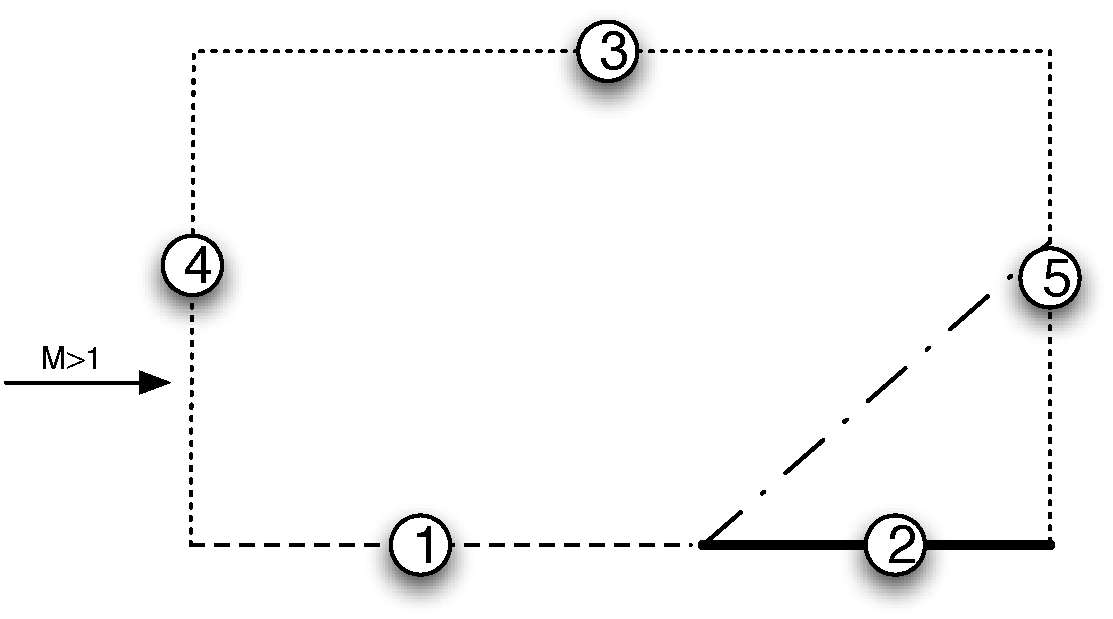
\includegraphics[scale=.5]{figs/flat_plate_BCs.pdf}
\caption{Carter flat plate problem.}
\end{figure}

\begin{itemize}
\item \textbf{Inflow boundary conditions:} free stream conditions are applied here to all four fluxes $\widehat{f}_{i,n}$.
\item \textbf{Symmetry boundary conditions:} $u_n = q_n = \pd{u_s}{n} = 0$. Here, this implies $u_2 = q_2 = \sigma_{12} = 0$. We impose the stress condition by noting that, for the flat plate geometry, if $u_2 = 0$, then at the top and bottom, with $n = (0,1)$, $\widehat{f}_{2,n} = \sigma_{12}$, and $\widehat{f}_{4,n} = q_2$ if $\sigma_{12}$ and $u_2 = 0$. 
\item \textbf{Flat plate boundary conditions:} $u_1 = u_2 = 0$, and $T = T_w = \left[1+(\gamma-1)M_\infty^2/2\right] T_\infty = 2.8T_\infty$ (for Mach 3 flow). We impose these strongly on the trace variables $\widehat{u}_1, \widehat{u}_2, \widehat{T}$. 
\item \textbf{Outflow boundary conditions:} the exact boundary conditions to enforce here are not universally agreed on.  Many enforce $\pd{u_1}{n}=\pd{u_2}{n}=0$ and $\pd{T}{n} = 0$, while others enforce an outflow boundary condition only in regions where the flow is subsonic.\cite{Demkowicz:1990:NFE:112271.112276}.  We adopt a ``no boundary condition'' outflow condition, first introduced in \cite{FLD:FLD1650140506}. A mathematical analysis and explanation of this boundary condition for standard $H^1$ elements is given in \cite{FLD:FLD505}. 

%An alternative boundary condition would be as follows: since $u_1$ and $u_2$ are not expected to be zero at these points, we can set $\widehat{f}_{2,n}$ and $\widehat{f}_{4,n}$ to their represented quantities using either the field variables from the background flow, or (in the case of pseudo-time stepping) the previous timestep's flux and field quantities. 

\end{itemize}

We initialize our solution to
\[
\rho = 1,\qquad u_1= 1,\qquad u_2 = 0, \qquad T = 1
\]
which is consistent with what was done in Demkowicz and Oden in \cite{Demkowicz:1990:NFE:112271.112276}. Stresses are set uniformly to zero. 

We take the computational domain to be $\Omega = [0,2]\times[0,1]$. We begin with a mesh of 8 by 16 elements. Under Dirichlet wall boundary conditions for all 3 traces $u_1$, $u_2$, and $T$, the solution develops a singularity in the density $\rho$ at the plate beginning, and both $T$ and $u_1$ form a boundary layer along the leading edge of the plate. Due to the presence of the singularity, the solution for $\rho$ is scaled such that the features of the solution away from the singularity are visible in Figure~\ref{fig:rhoScaled}.

\begin{figure}[!h]
\centering
\subfigure[$\rho$]{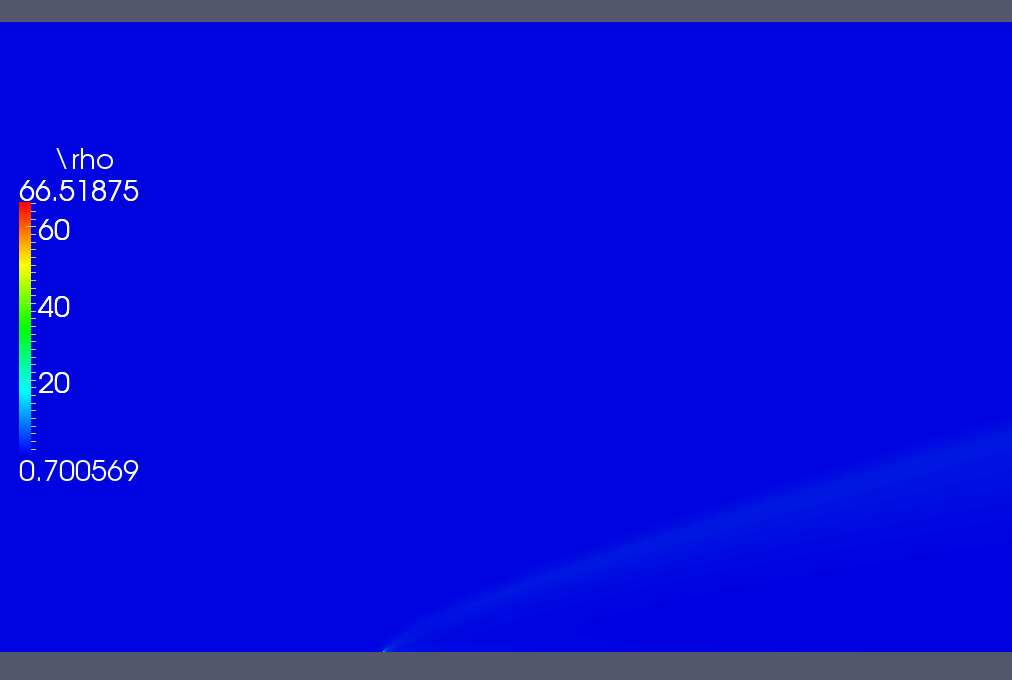
\includegraphics[scale=.21]{figs/Re1000p2/rhoUnscaled.png}}
\subfigure[$u_1$]{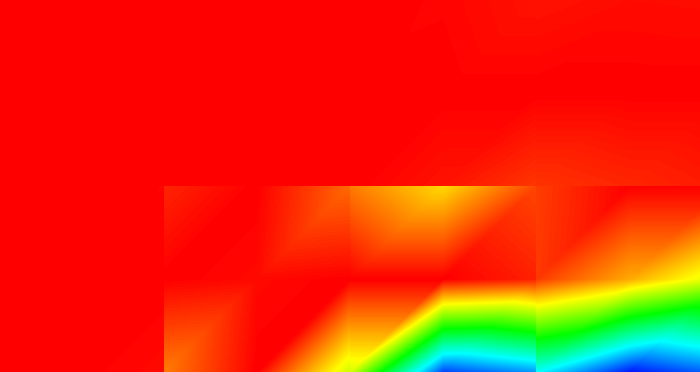
\includegraphics[scale=.21]{figs/Re1000p2/u1.png}}
\subfigure[$u_2$]{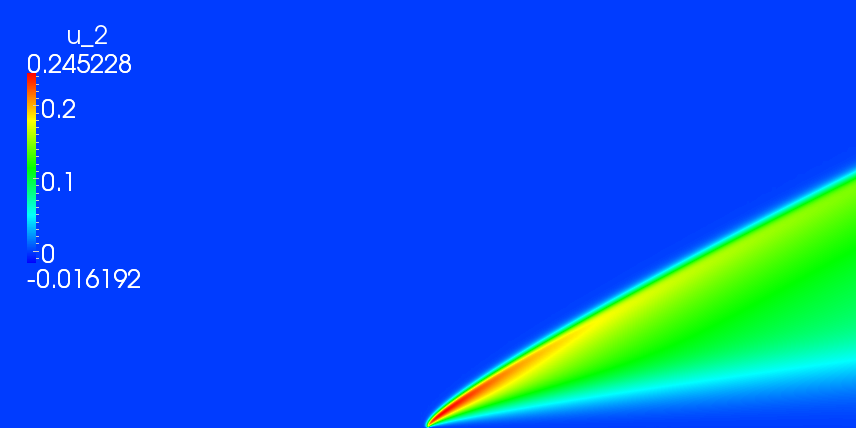
\includegraphics[scale=.21]{figs/Re1000p2/u2.png}}
\subfigure[$T$]{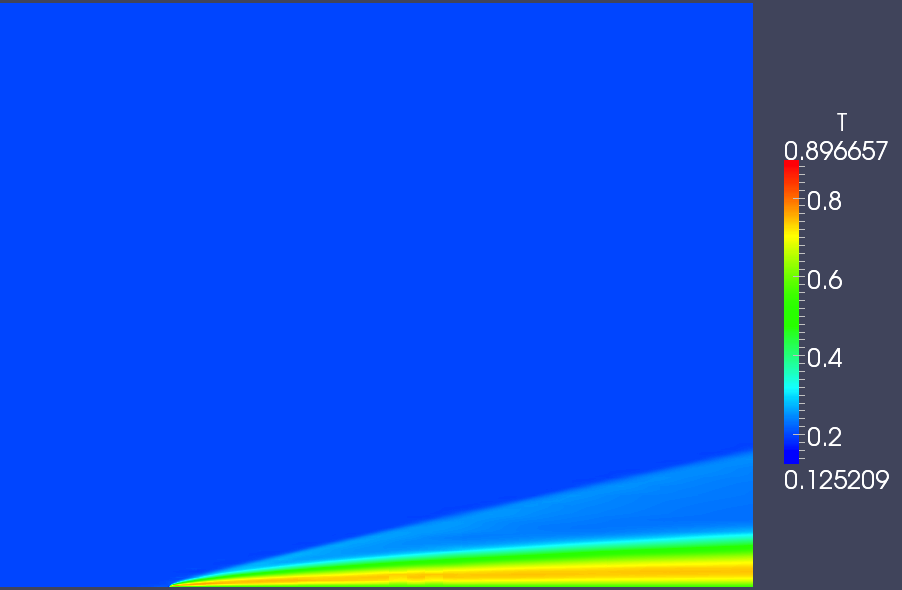
\includegraphics[scale=.21]{figs/Re1000p2/T.png}}
\caption{Solutions after seven refinements for $p=2$ and $\Reyn = 1000$.}
\label{fig:Re500}
\end{figure}

\begin{figure}[!h]
\centering
\subfigure[$\rho$]{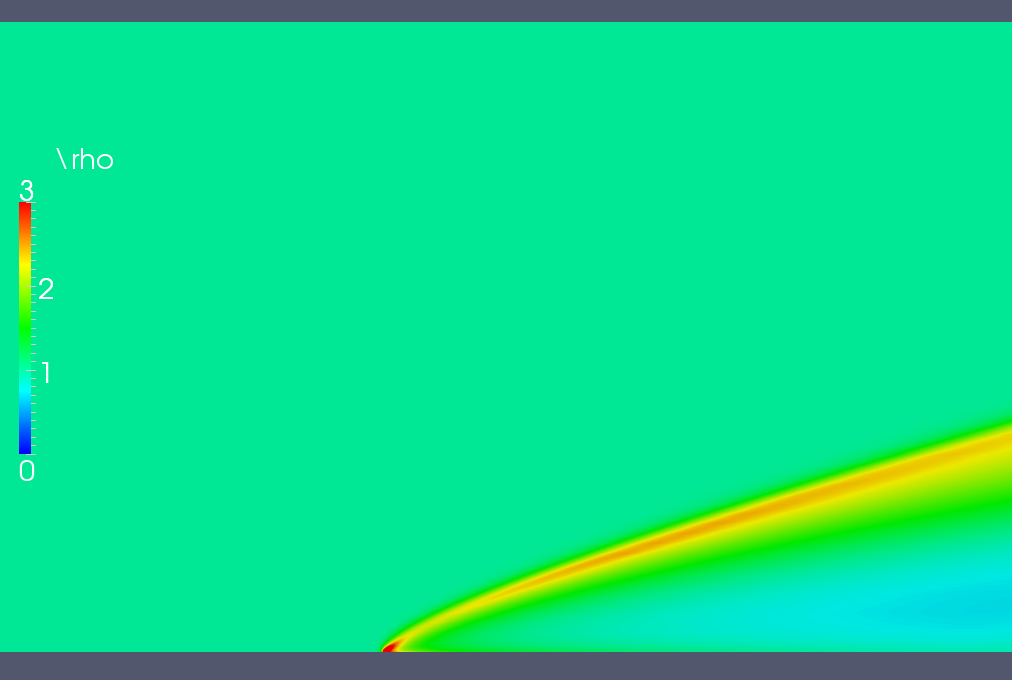
\includegraphics[scale=.25]{figs/Re1000p2/rhoScaled.png}}
\subfigure[Mesh]{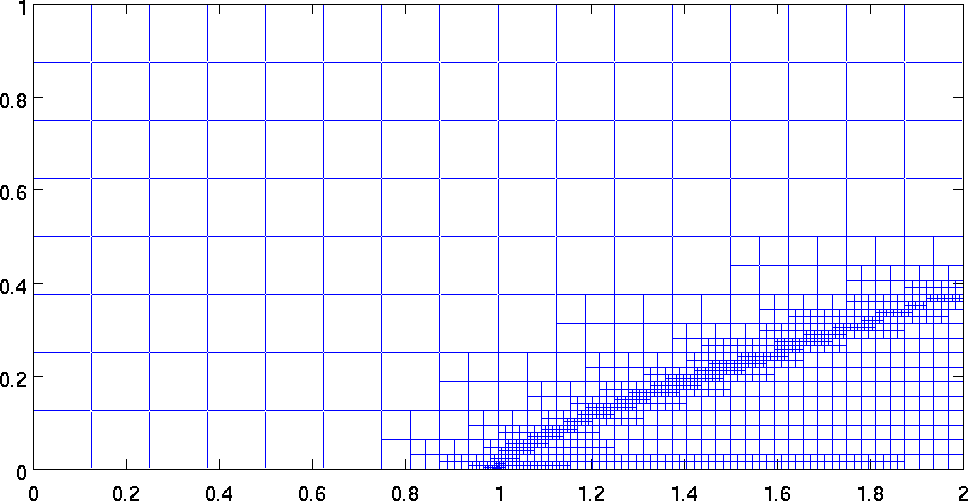
\includegraphics[scale=.57]{figs/Re1000p2/mesh6.png}}
\caption{Rescaled solution for $\rho$ in the range $[0,3]$ and adaptive mesh after seven refinements.}
\label{fig:rhoScaled}
\end{figure}

\begin{figure}[!h]
\centering
\subfigure[$\rho$]{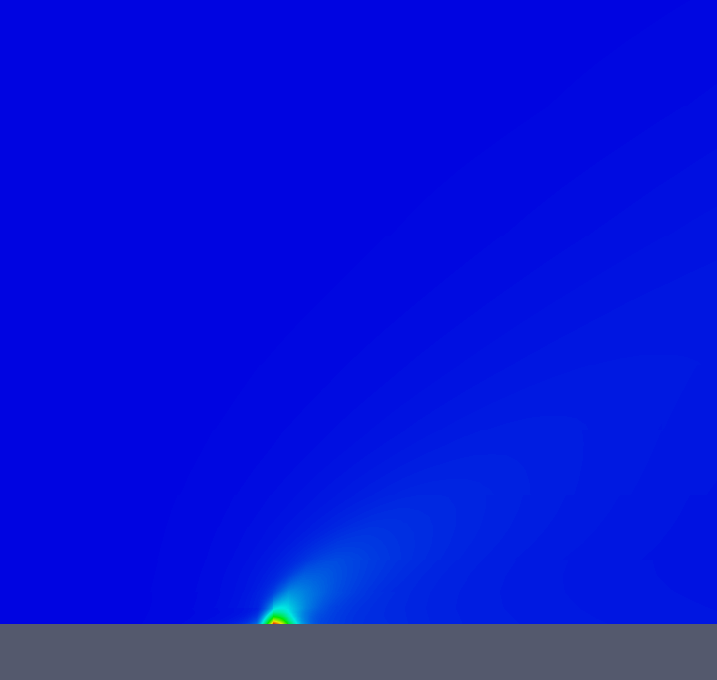
\includegraphics[scale=.23]{figs/Re1000p2/rhoUnscaledzoom.png}}
\subfigure[$u_1$]{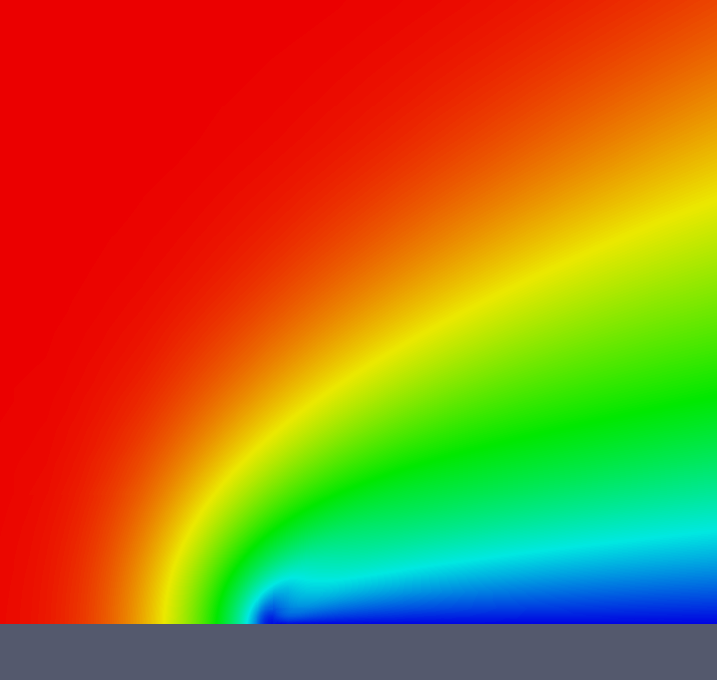
\includegraphics[scale=.23]{figs/Re1000p2/u1zoom.png}}
\subfigure[$u_2$]{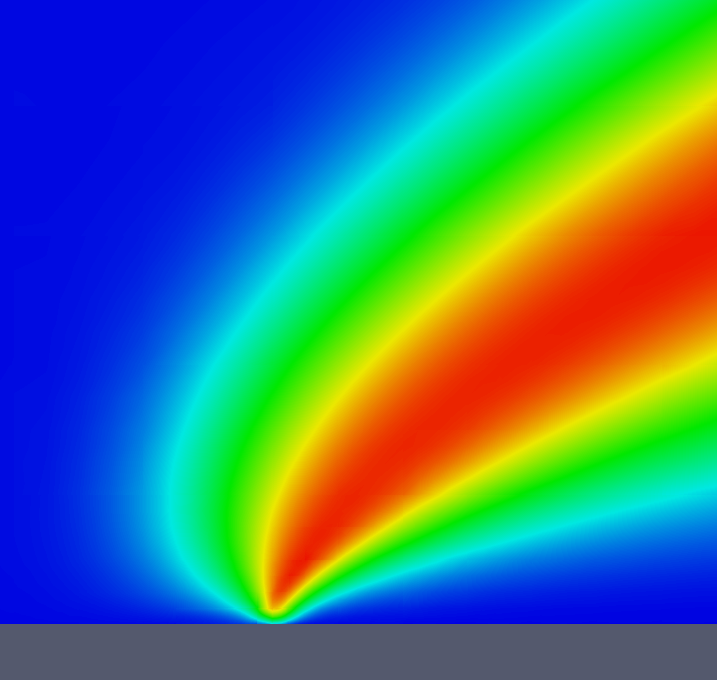
\includegraphics[scale=.23]{figs/Re1000p2/u2zoom.png}}
\subfigure[$T$]{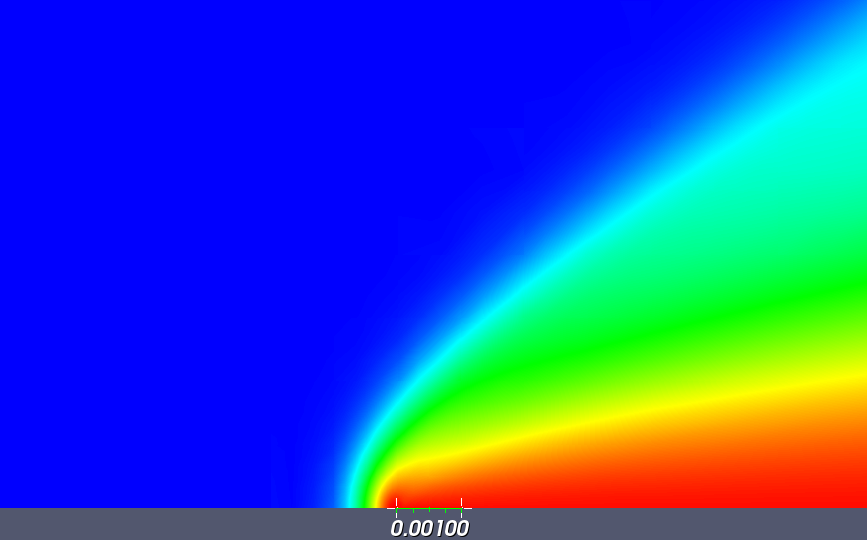
\includegraphics[scale=.23]{figs/Re1000p2/Tzoom.png}}
\caption{Zoom of solutions at the beginning of the plate for $p=2$ and $\Reyn = 1000$.}
\end{figure}

\begin{figure}[!h]
\centering
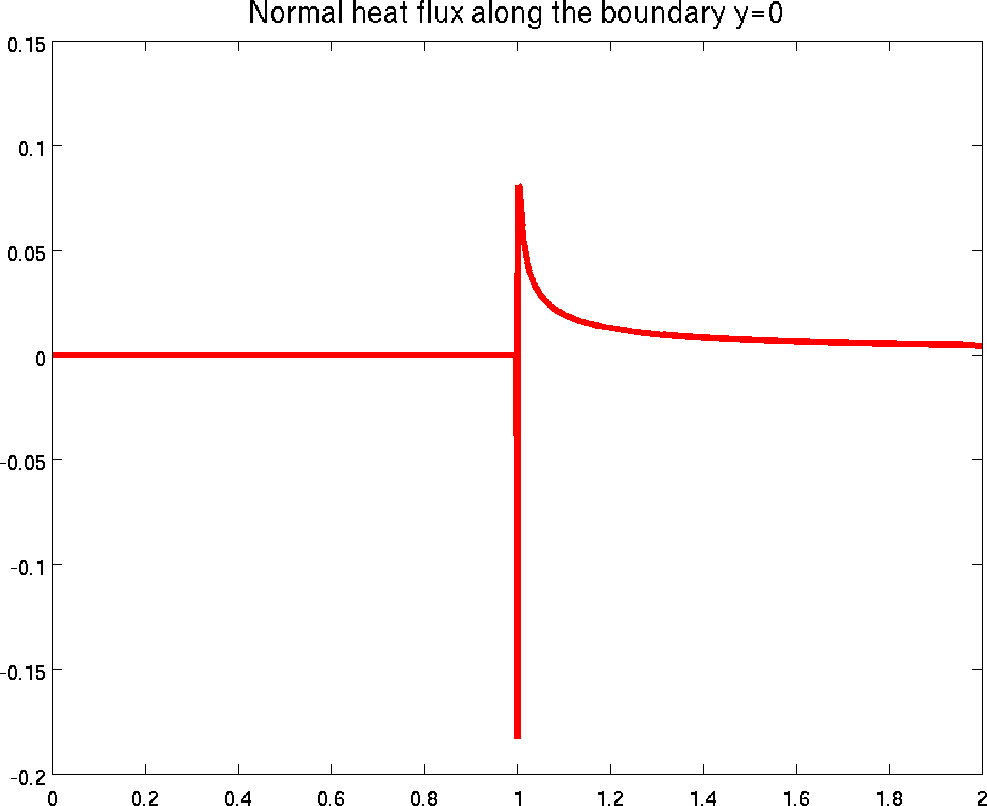
\includegraphics[scale=.45]{figs/Re1000p2/heatflux.png}
\caption{Heat flux at the bottom boundary.}
\end{figure}


\section{Conclusions and future work}

The goal of this work has been to explore the behavior of the Discontinuous Petrov-Galerkin (DPG) method as a method for the discretization and solution of convection-dominated diffusion problems, and to produce both theory and numerical results for model problems in this area.  We begin by introducing the DPG method for linear problems; the concept of problem-dependent optimal test functions is derived through equivalence with the minimization of a specific residual, and discontinuous test functions are introduced in order to localize the determination of such optimal test functions to a single element.  

The DPG framework is then extended to nonlinear problems, and equivalence is shown between the DPG method and a Gauss-Newton minimization scheme for the nonlinear residual.  An anisotropic refinement scheme is implemented to more effectively capture lower-dimensional behavior of solutions of convection-diffusion problems, such as boundary layers.  We extrapolate the DPG method to a nonlinear viscous Burgers' equation, and conclude by applying the DPG method to systems of equations and to the solution of two model problems in viscous compressible flow.  

In particular, we demonstrate for both the flat plate and compression ramp problem in supersonic/hypersonic in compressible flow that the DPG method is able to begin from a highly underresolved meshes (two elements for the Carter plate problem, and 12 elements for the Holden ramp problem), and resolve physical features of the solution through automatic adaptivity, without the aid of artificial diffusivity or shock capturing terms.  We believe this indicates both the robustness of the method on coarse grids and the effectiveness of the DPG error indicator for adaptive refinement.  

As is the case with any research, much work remains to be done.  We have chosen the classical variables in which to cast the compressible Navier-Stokes equations; however, investigation of alternative sets of variables may have merit, as different choices of variables yield differing linearizations with their own advantages (for example, all derivatives in time are linear with respect to the momentum variables, and the entropy variables of Hughes both symmetrize the Navier-Stokes equations and yield solutions obeying second law of thermodynamics for standard $H^1$ formulations \cite{Hughes1986223}).  

We also hope to investigate artificial viscosity methods as regularization for problems in viscous compressible flow.  We present an analysis of the 1D Burgers' equation demonstrating that the exact solutions under Newton linearization contain large oscillations.  While these oscillations are not the result of the stability of the spatial discretization, their presence can cause density and temperature to become non-physically negative, which can stall the convergence of the nonlinear solver.  Our goal in incorporating artificial viscosity would not be to provide additional stabilization mechanisms for the discrete spatial discretization, but to provide regularization with which to suppress the presence of large oscillations in the linearized solution.  

Finally, though the method is inf-sup stable for arbitrary meshes, our experiments have focused on meshes of uniform $p$.  We hope to implement a true $hp$-adaptive DPG method in the future.  

%\bibliographystyle{plain}
\bibliographystyle{unsrt}
\bibliography{paper,NSNotes,DPGarticles}

\end{document}
